\documentclass[9pt,twocolumn,twoside]{pnas-new}
\usepackage{subfigure}
% Use the lineno option to display guide line numbers if required.
% Note that the use of elements such as single-column \emph{?}quations
% may affect the guide line number alignment.

\usepackage{color}

\templatetype{pnasresearcharticle} % Choose template
% {pnasresearcharticle} = Template for a two-column research article
% {pnasmathematics} = Template for a one-column mathematics article
% {pnasinvited} = Template for a PNAS invited submission

\title{Pathways to Climate, Weather, and Environmentally Related Protest Events}

% Use letters for affiliations, numbers to show equal authorship (if applicable) and to indicate the corresponding author
\author[a,1]{Fang Jin}
\author[a]{Wei Wang}
\author[a]{Brian J. Goode}
\author[a]{Chang-Tien Lu}
\author[a]{Naren Ramakrishnan}

\affil[a]{Discovery Analytics Center (Dept. of Computer Science), Virginia Tech - NCR, Arlington, VA 22203}

% Please give the surname of the lead author for the running footer
\leadauthor{Jin}


\significancestatement{From 1995-2015, 90\% of global disasters are caused by extreme weather events such as flood, storm, heat wave and so on. What is more, the extreme weather events are increasing continuously, resulting natural disasters happen more and more frequent. Records from the international disaster database EM-DAT shows, the average disasters per year from 2005 to 2014 is 14\% higher than the years between 1995 and 2004, and is twice of years between 1985 and 1994. However, how the extreme weather events lead to armed conflicts is still under disclosed. This work presents a promising strategy to identify climate change related protests in South America, and further trace back protest causalities, and discover the mainly evolution patterns from climate change to civil unrest. This work can be extended into United States and other countries, to help decision makers understand the evolution path from extreme weather events to civil unrest, and benefit for society stabilization and human well-beings.}


% Please include corresponding author, author contribution and author declaration information
\authorcontributions{Please provide details of author contributions here.}
\authordeclaration{Please declare any conflict of interest here.}
\correspondingauthor{\textsuperscript{1}To whom correspondence should be addressed. E-mail: jfang8@vt.edu}

% Keywords are not mandatory, but authors are strongly encouraged to provide them. If provided, please include two to five keywords, separated by the pipe symbol, e.g:
\keywords{Climate change $|$ Extreme weather $|$ Civil unrest $|$ Evolution Pattern}


\begin{abstract}
\textit{Abstract goes here.}
\end{abstract}

\dates{This manuscript was compiled on \today}
\doi{\url{www.pnas.org/cgi/doi/10.1073/pnas.XXXXXXXXXX}}

\begin{document}

% Optional adjustment to line up main text (after abstract) of first page with line numbers, when using both lineno and twocolumn options.
% You should only change this length when you've finalised the article contents.
\verticaladjustment{-2pt}

\maketitle
\thispagestyle{firststyle}
\ifthenelse{\boolean{shortarticle}}{\ifthenelse{\boolean{singlecolumn}}{\abscontentformatted}{\abscontent}}{}
\section{1. Introduction}
\dropcap{C}limate change, extreme weather, and the state of the environment directly impact the availability of food \cite{RW3}, energy \cite{}, and shelter \cite{}.
As finite resources become scarce, the residual impacts on local economies can have disastrous and long-lasting effects on the fundamental livelihoods of inhabitants for decades \cite{}.
In some cases, the resulting instability can severely detriment the ability of an established political system to maintain peace.
The examples of this occurring are numerous.
The extended drought in Syria in 2011 is cited as one of the principle causes of civil war \cite{gleick2014water,kelley2015climate}.
In a smaller scale example, the environmental impact of lead contamination in the drinking water in the United States led to protests in 2016.
The extreme weather event, Hurricane Manuel, that devastated the western coasts of Mexico led to subsequent protests over resources at points as long as 1 year after the initial event.

Of course, the occurrence of either a shift in climate, extreme weather, or environmental catastrophe is not sufficient to guarantee that civil unrest is likely to follow.
In general the causal mechanisms leading to civil unrest are very complex, and there is no easy way to determine a linear pathway to protest.
However, to date, little quantitative analysis has been performed on the residual effects of changes resulting from climate, extreme weather, and the environment using a large volume of data.
In this analysis, we focus on the breadth of the climate events by looking at events generated from a large Gold Standard Report (GSR) containing all of the protests that have occurred in Latin America from 2011-2013.
By developing a logistic regression classifier, 25352 GSR civil unrest events were classified as either being climate or non-climate related using terms in the description of the event.


NEXT... WHAT DID WE FIND???
{\color{red}
NOTE: THERE ARE A LOT OF FIGURES - these are observations - BUT WE NEED TO DRAW CONCLUSIONS. WHAT DO YOU LEARN FROM THESE FIGURES? HOW CAN YOU MAKE QUANTIFIABLE COMPARISONS? WHAT INTERESTING THINGS DO YOU FIND IN THE DATA. CURRENTLY, THERE IS SPATIAL, (TEMPORAL?), and ``CAUSALITY''. PLEASE TRY TO THINK ABOUT WAYS TO CHARACTERIZE THE DIFFERENCES/SIMILARITIES BETWEEN CLIMATE/NON-CLIMATE PROTESTS. ALSO, HOW WOULD YOU COMPARE ACROSS THE 3 COUNTRIES YOU'VE ANALYSED?}

\begin{itemize}
  \item First, we develop a logistic regression classifier, which can classify climate protests from non-climate protests automatically based on protest events description.
  \item Second, we analyze the climate protest spikes and disclose its relationship with climate disasters. For example, we plot the climate protests time series in Mexico and Brazil, and overlay with corresponding climate disasters, found for storm and hurricane events in Mexico, the protest time line last much longer. However, for drought events in Brazil, the protests being initiated more swift, also last shorter time.
  \item Thirdly, we figure out the proportion of protest causality. By studying some major climate disasters, we also discover each protest category's demands.
  \item Finally, We investigate the climate cocurrence. For instance, the water related protests are often accompanies with electricity shortage.
while land protest are often isolated reasons.
\end{itemize}
%

%

%
%
\section{2. Related research}
The path from climate, extreme weather and environmental effects to civil unrest is causally complex \cite{hsiang2011civil,RW5} and involves various combinations of climate change \cite{burke2014climate}, natural resources, human security, and social stability.
In general, sensitivities to climate change, exposure to climate change, and the ability of a society to adapt are indicators of whether or not violence will erupt~\cite{RW9}.
A commonly studied pathway is the effect of climate on food prices which then induces civil unrest.
An examples of this occurrence is the Arab Spring uprisings in 2011, and how weather effects food prices~\cite{RW2}.
The pathway to civil unrest is also not limited to a local region, where one study shows the Chinese drought effecting the supply wheat causing prices to rise in the Egyptian break market leading to protest~\cite{RW1}.
The pathways of food prices to protest have also been studied in the global south~\cite{RW4}, Africa, and Asia~\cite{wischnath2014climate,RW6}.
However, even this path of climate effects on income level leading to conflict is not eminently clear~\cite{RW10}.

{\color{red} This second paragraph will discuss work more related to the specific conclusions that we draw... we don't have these yet. Or do we? Anyway cite Hsiang here...}

{\color{red} Protest work w/ EMBERS and related programs. Tools available for use. Brian to add in using text/refs similar to his other protest papers.}



\section*{3. Climate Protests Overview}

\begin{figure}[ht]
\centerline
{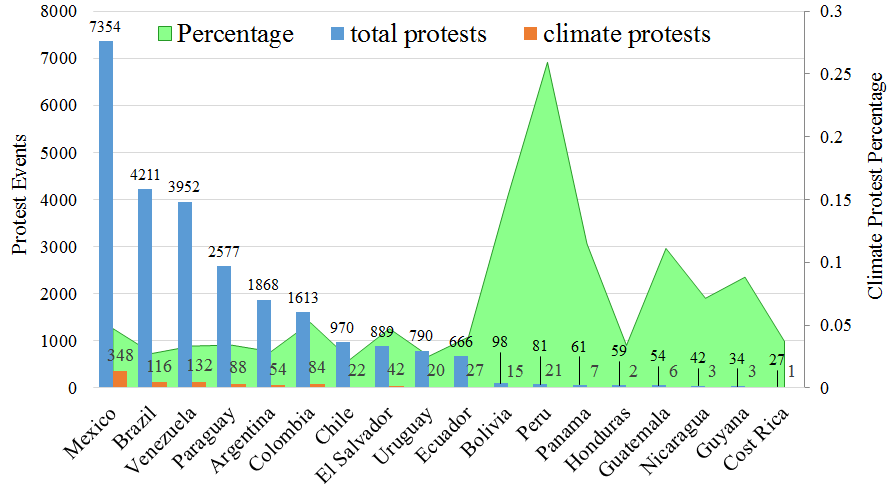
\includegraphics[width=.45\textwidth]{figures/month-country-protest3}}
\caption{Blue bar shows all the GSR protest events, yellow bar shows climate related protest events, green area shows the climate protest percentage over all the Latin American countries, from July 2012 to March 2015.}
\label{month_percentage}
\end{figure}


\begin{figure}[ht]
\centerline
{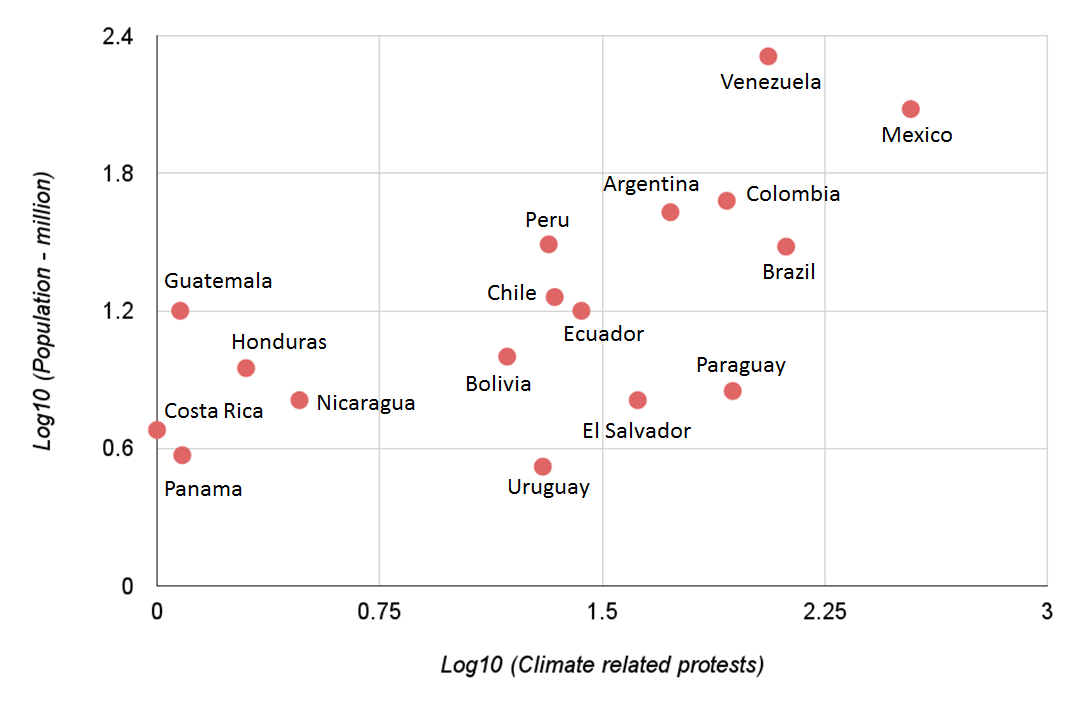
\includegraphics[width=.4\textwidth]{figures/protest-population}}
\caption{Climate protest events and population (million) of each country. The two series have a Pearson correlation coefficient 0.64.}
\label{protest-population}
\end{figure}


\begin{figure}[ht]
	\centering
	\subfigure[]{
		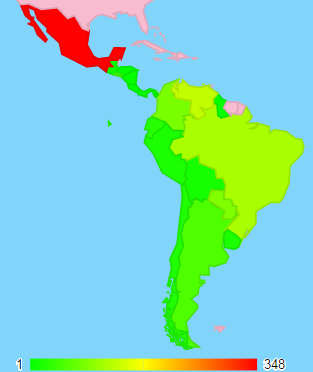
\includegraphics[height=1.5in] {figures/map-climate-number}
		\label{map_number}
	}
	\subfigure[]{
		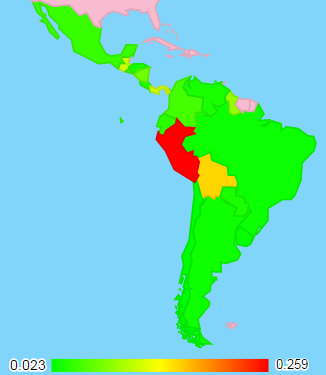
\includegraphics[height=1.5in] {figures/map-climate-percentage}
		\label{map_percentage}
	}
	\caption{(a) Climate related protests events numbers; (b) Climate related protests percentage in Latin American countries, from July 2012 to March 2015. }
\label{map}
\end{figure}


We study 25352 GSR civil unrest events across Latin American countries from July 2011 to March 2015. We build a climate change protest classifier, aim to identify how many civil unrest events are caused by climate change or extreme weathers. Among all the 25352 GSR protest events,  991 events are classified into climate-related events. In other words, in Latin American countries, the climate related protests accounts for 3.91\%. As shown in Figure~\ref{month_percentage}, Blue bar shows all the GSR protest events, from the highest amount of Mexico 7354 to lowest country Cost Rica 27; yellow bar shows climate related protest events; the blue area describes the climate related protests percentage over all the GSR protest events. Figure~\ref{map_number} plots the climate related protests events numbers, we can see Mexico has the most climate protests events, as high as 348. And Figure~\ref{map_percentage} gives us a straight view of climate protest percentage, of which, Peru climate protest accounts as high as 25.9\%, Bolivia climate protest percentage reaches as high as 15.3\%, Panama 11.4\% and Guatemala 11.1\% respectively.

Countries like Mexico, Brazil, and Venezuela have both high none-climate and climate protests, and their climate percentile rates are roughly stable around 4 \%.
We pull out these three countries' climate and non-climate events location, and show their distribution on the map, as shown in Figure~\ref{climate-map}. Interestingly, climate protests in Brazil mainly center at two major cities, Sao Paulo, and Rio de Janerio. While for Mexico and Venezuela, the climate protest city happens in most cities uniformly. Probably, it is because that the climate protest distribution is closely correlated with population density, the higher population density area, the more protest events, regardless of climate or non-climate. We can also see from Figure~\ref{month_percentage}, countries like Panama, Honduras, Nicaragua, Guyana and Cost Rica, have both low none-climate and climate protests. This is probably because these countries have smaller population, suffer less natural disasters, and better governance.


We investigate the protest event time series in South American. As shown in Figure 3, on average, February, March, and May see the most climate-related protest events, while November has the less. We can also see the for the none-climate protest, the temporal distribution is different since it see most protest in July. This is because there are more climate disasters than other months. This is consist with the statistic data concerning the natural disasters in South American.

\begin{figure*}[ht]
	\centering
    \subfigure[Mexico]{
		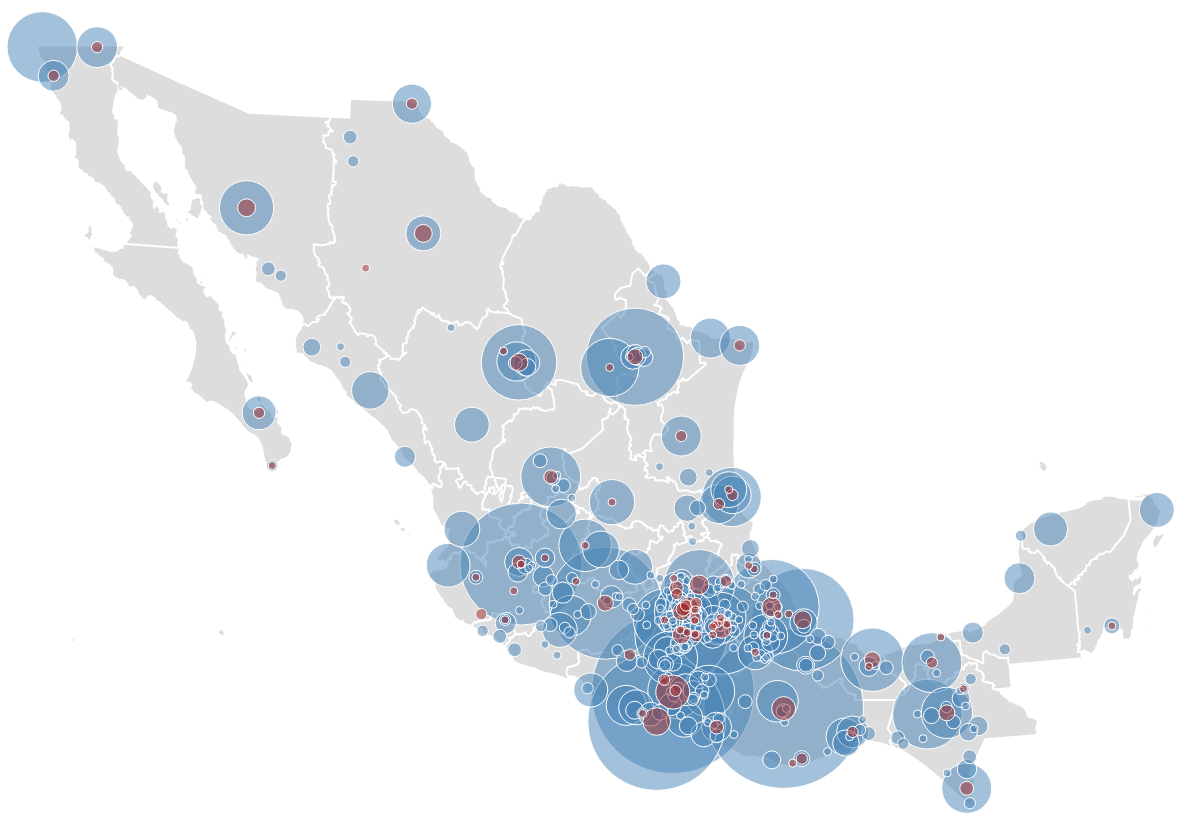
\includegraphics[height=1.4in] {figures/Mexico_climate_non-climate}
		\label{Mexico_map}
    }
	\subfigure[Brazil]{
		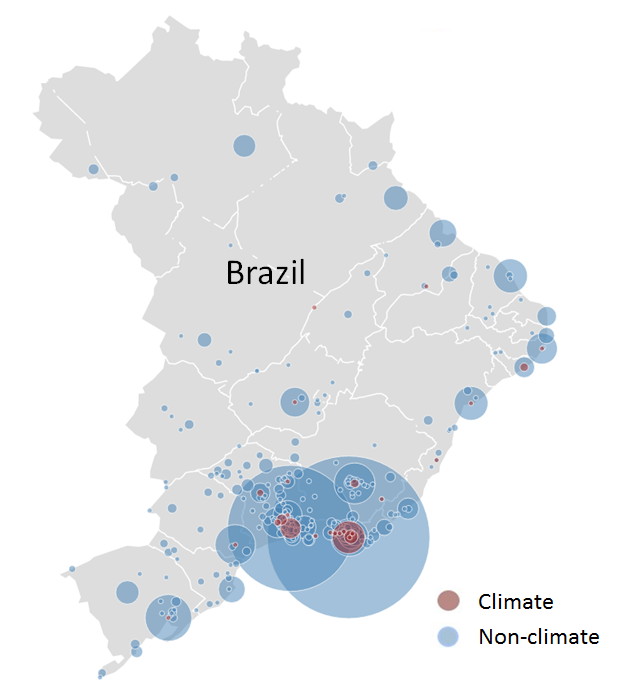
\includegraphics[height=1.6in] {figures/Brazil}
		\label{Brazil_map}
	}
	\subfigure[Venezuela]{
		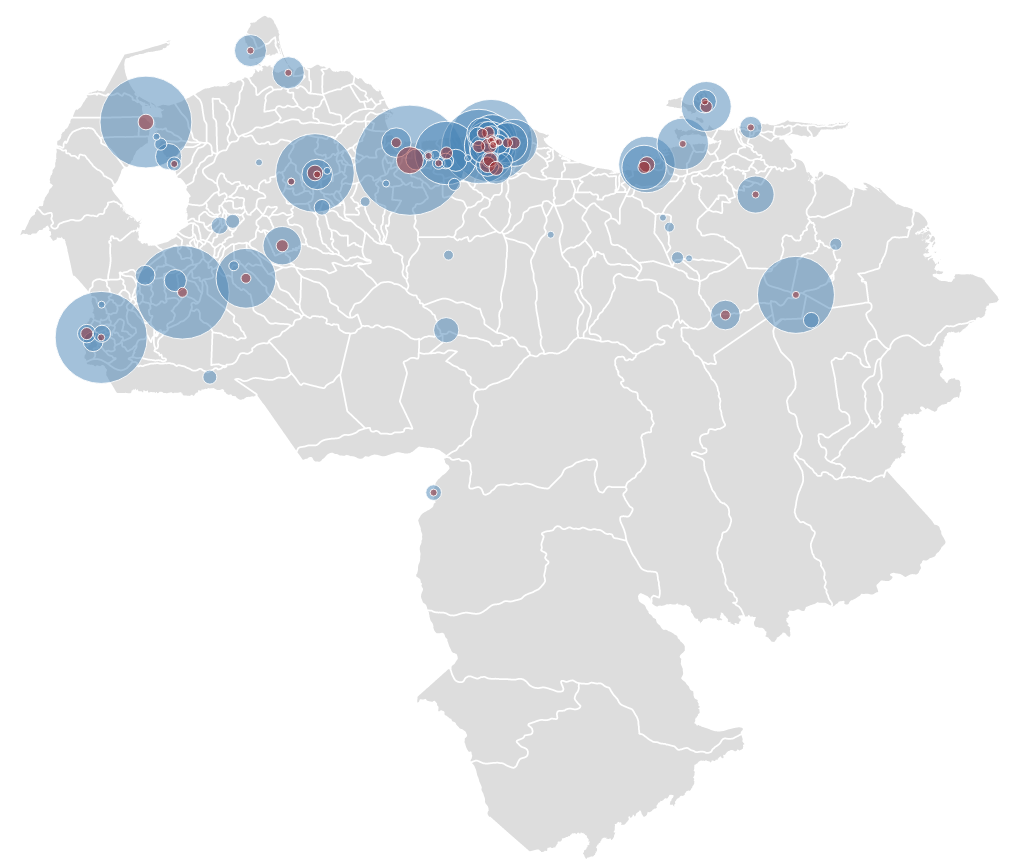
\includegraphics[height=1.5in] {figures/Venezuela_climate_non-climate}
		\label{Venezuela_map}
	}
	\caption{Climate and non-climate protests from July 2012 to March, 2015. Red circle represents climate related protest events, and blue circle represents non-climate related protests. }
\label{climate-map}
\end{figure*}


%\begin{figure}[ht]
%	\centering
%	\subfigure[]{
%		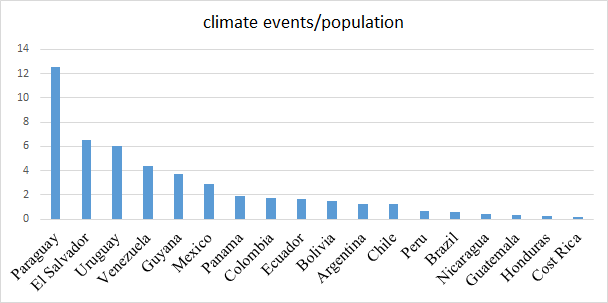
\includegraphics[height=1.25in] {figures/climate_events_per_population}
%		\label{population}
%	}
%	\subfigure[]{
%		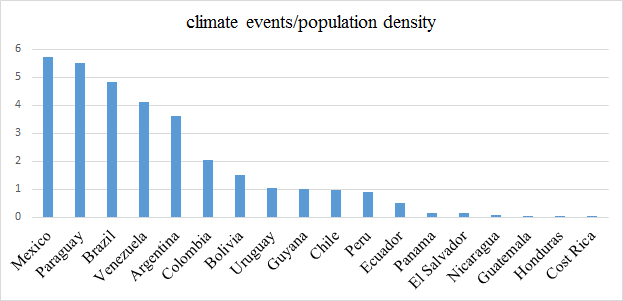
\includegraphics[height=1.25in] {figures/climate_events_per_population_density}
%		\label{population-density}
%	}
%	\caption{(a) Climate protest events as per population of each country; (b) Climate protests per population density of each country. }
%\label{population-density}
%\end{figure}



%\subsection{3.3 Protest time interval deviation}
%Figure~\ref{Mexico-deviation} shows Mexico climate and non-climate protests time interval distribution. We found the non-climate protests have very high percentage with small time interval, less than three days. The climate protests, on the contrary, time interval is longer than non-climate protests.
%
%\begin{figure}[ht]
%\centerline
%{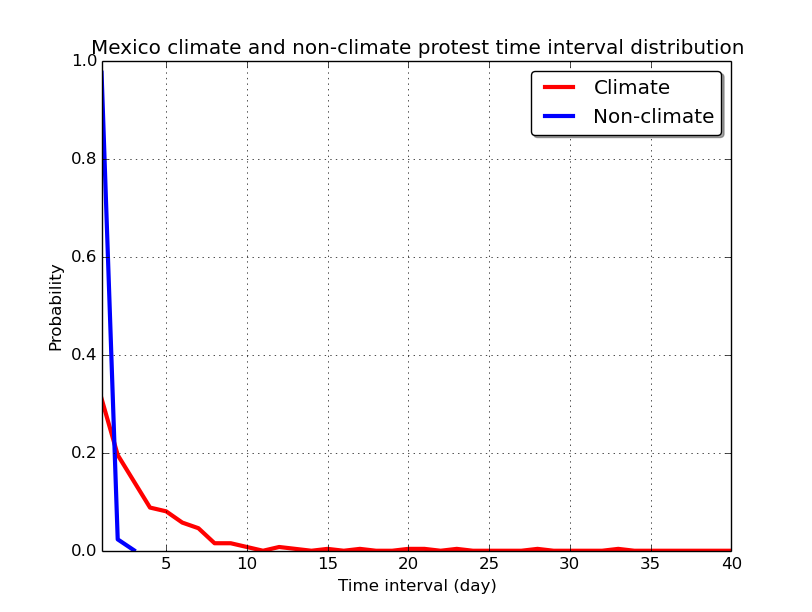
\includegraphics[width=.3\textwidth]{figures/Mexico_deviation}}
%\caption{Mexico climate and non-climate protests time interval deviation. Blue curve shows the non-climate protest time intervals percentage, and red curve shows climate protest time interval percentage.}
%\label{Mexico-deviation}
%\end{figure}


\begin{figure*}[ht]
	\centering
	\subfigure[Mexico]{
		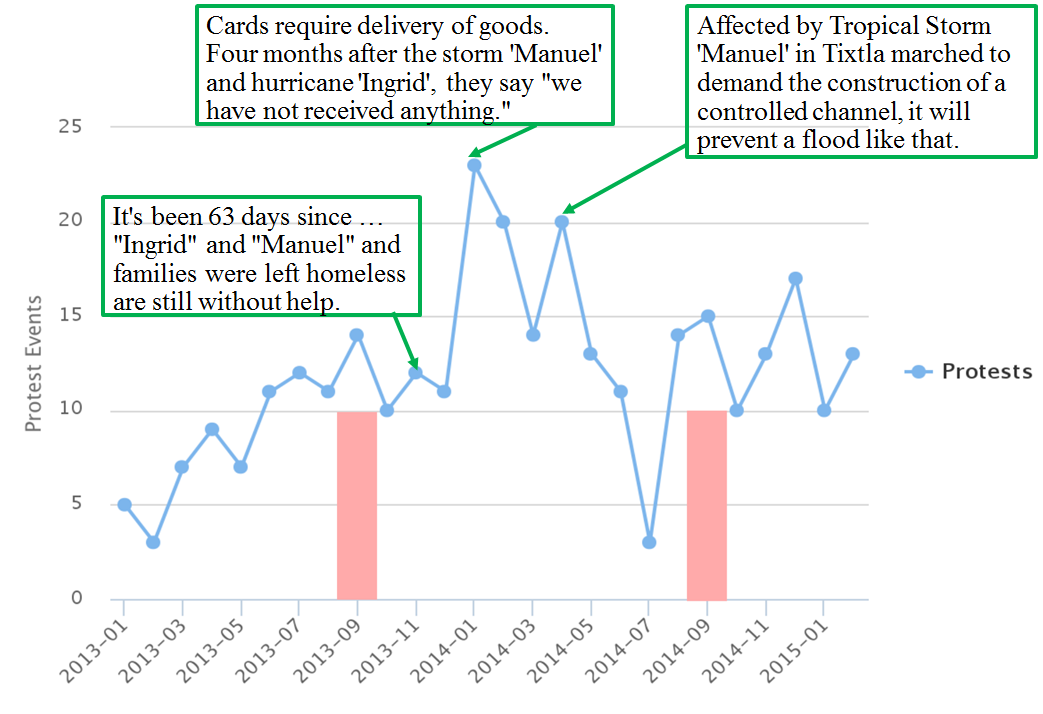
\includegraphics[height=1.3in] {figures/Mexico_disaster2}
		\label{Mexico_disaster_timeseries}
	}
	\subfigure[Brazil]{
		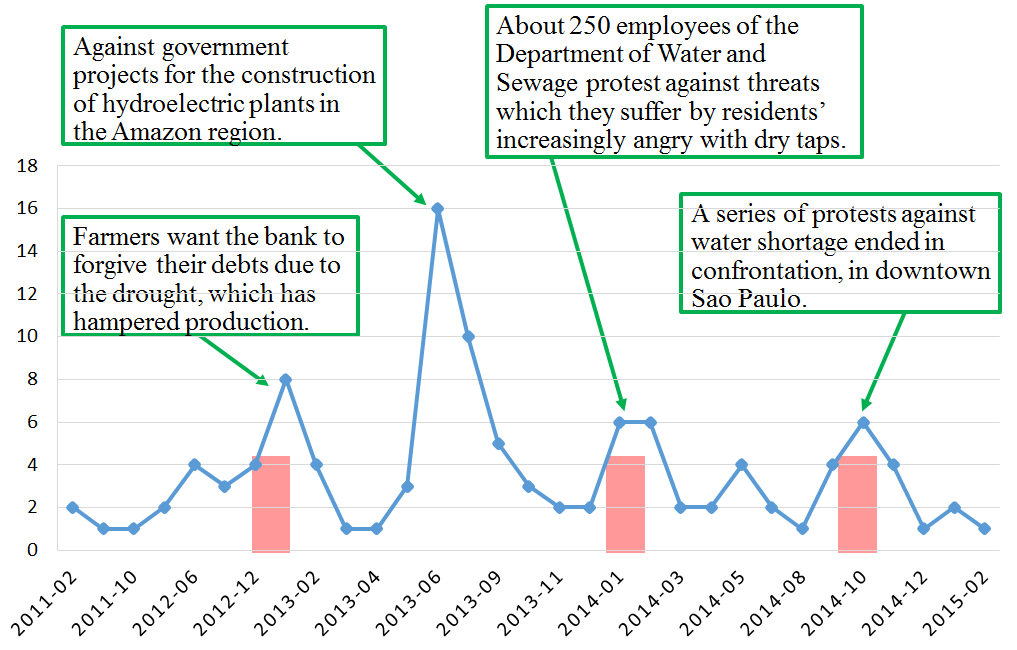
\includegraphics[height=1.3in] {figures/Brazil_disaster1}
		\label{Brazil_disaster_timeseries}
}
	\subfigure[Venezuela]{
		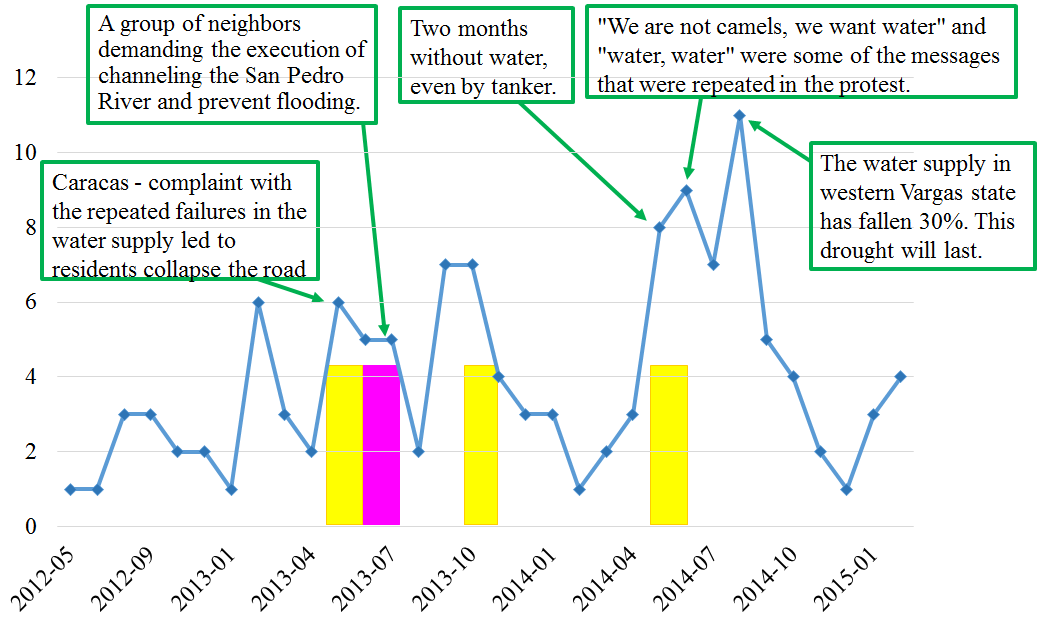
\includegraphics[height=1.3in] {figures/Venezuela_disaster}
		\label{Venezuela_disaster_timeseries}
	}
	\caption{(a) Mexico climate disasters and climate protests. The blue time series shows the climate related protest events, and light red vertical lines show two storm diasters in Mexico, storm Manuel in September 17, 2013 and hurricane Odile in September 15, 2014 respectively. (b)Brazil climate disasters and climate protests. The blue time series shows the climate related protest events, and yellow vertical lines show three drought diasters in Brazil, drought in Feb 2012, Heat wave in Feb 2014, and drought in Oct 2014, respectively. (c) Venezuela climate disasters and climate protests. The blue time series shows the climate related protest events, and rose vertical line show local area flood diaster, and yellow vertical lines drought disasters.}
\label{climate-timeseries}
\end{figure*}


\subsection{4. Climate disasters and climate protests}
For the climate protests, we intend to find out what kind of climate disasters trigger them, What is the interaction between climate change and civil unrest, and how is the character of time span for different climate events. With the aid of International Disaster Database EMDAT~\footnote{http://www.emdat.be/database}, World Disasters Timeline~\footnote{http://www.mapreport.com/} and European Commission's Humanitarian Aid and Civil Protection department (ECHO)~\footnote{http://ec.europa.eu/echo/}, we query the official climate disaster report for each country and overlay with climate related protests, as shown in Figure~\ref{climate-timeseries}.


\paragraph{Mexico climate disasters}
Figure~\ref{Mexico_disaster_timeseries} shows Mexico climate disasters and protests, the blue time series represent the climate protests events, and the two red bar shows two storm disasters. The first red bar represents tropical storms Manuel (category 1) and Ingrid in September 17, 2013, whose track map can be seen in Figure~\ref{storm2013}. The storm Manael crossed west coast of Mexico, results in more than 23,000 people fled their homes due to heavy rains spawned by what had been Hurricane Ingrid, and 9,000 went to emergency shelters, at least 20 highways and 12 bridges had been damaged~\footnote{https://weather.com/storms/hurricane/news/tropical-storm-manuel-hurricane-ingrid-hit-mexico-opposite-coasts-20130916}.
After the storm Manuel, related protests and other civil unrest events break out dozens of times, and lasts for more than two years because the government's response had been desperately inadequate. The related protest reached climax in January 2014, and second climax in April 2014. We can see on November 19, 2013, there was report saying `it's been 63 days since the onslaught of `Ingrid' and `Manuel' and families were left homeless are still without help'. On January 22, 2014, news reporting `Cards require delivery of goods. Four months after the storm `Manuel' and the effects of Hurricane `Ingrid', they say `we have not received anything'. On April 7, protest description saying `Affected by Tropical Storm `Manuel' in the municipal head of Tixtla marched to demand the construction of a controlled channel, it will prevent a flood like that caused the overflow from the Black Lagoon in September 2013'. All those kind of protests caused by storm Manuel, we plot its descriptions in word cloud, as shows in Figure~\ref{Manuel_word_cloud}.

\begin{figure}[ht]
	\centering
	\subfigure[Storm Manuel, Sept 2013]{
		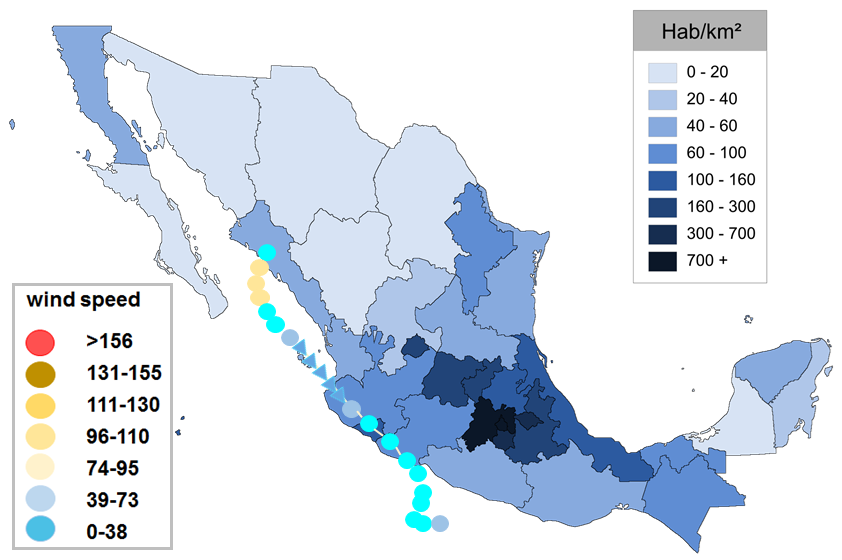
\includegraphics[width=1.55in] {figures/Mexico-2013-Manuel-new}
		\label{storm2013}
	}
	\subfigure[Hurricane Odile, Sept 2014]{
		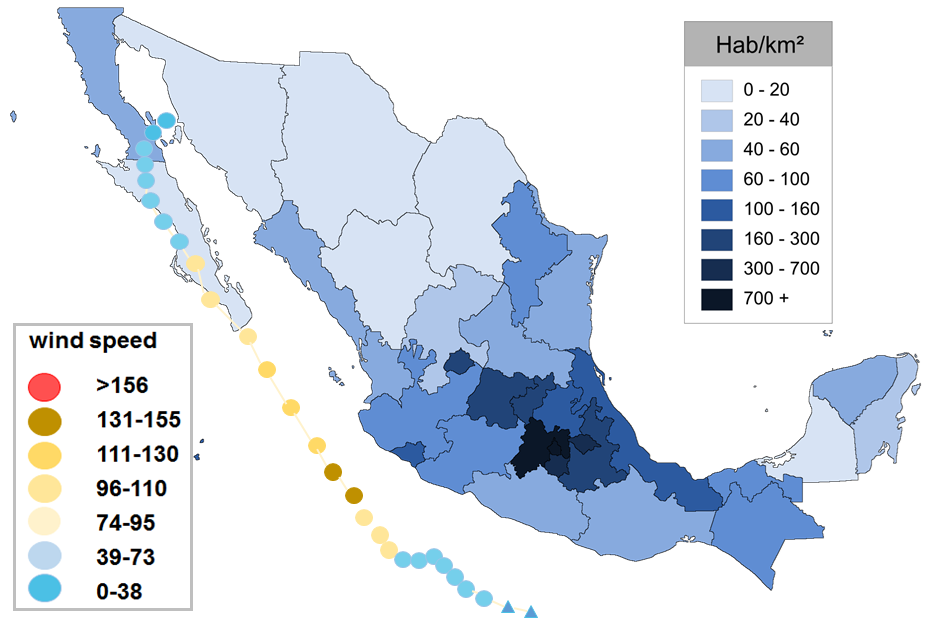
\includegraphics[width=1.55in] {figures/Mexico_2014_Odile-new}
		\label{storm2014}
	}
	\caption{Track map of Tropical Storm Manuel of the 2013 and Hurricane Odile of the 2014 Pacific hurricane season. The points show the location of the storm at 6 hour intervals. The colour represents the storm's maximum sustained wind speeds as classified in the Saffir Simpson hurricane wind scale, and the shape of the data points represent the nature of the storm. The map shows population density of all Mexico's 32 states. }
\label{Mexico-track-map}
\end{figure}


\begin{figure}[ht]
\centerline
{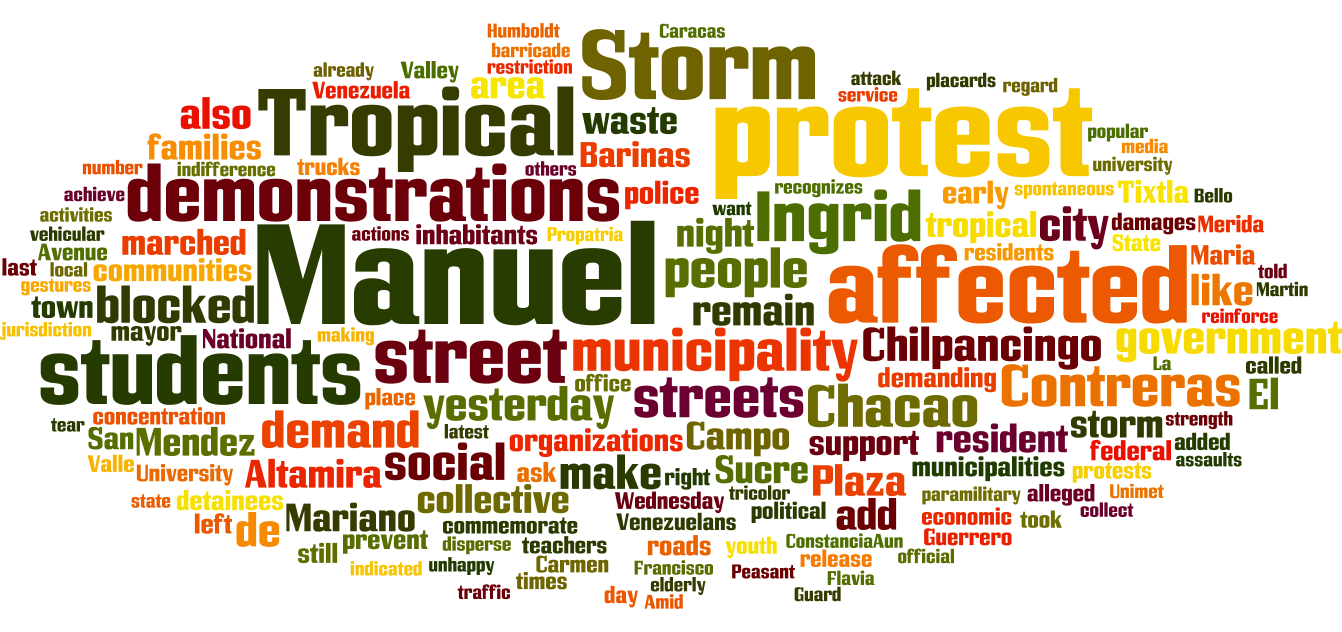
\includegraphics[width=.3\textwidth]{figures/Mexico_Manuel_wordcloud}}
\caption{Word cloud of Mexico storm Manuel, Sept 13, 2013.}
\label{Manuel_word_cloud}
\end{figure}


\begin{figure}[ht]
\centerline
{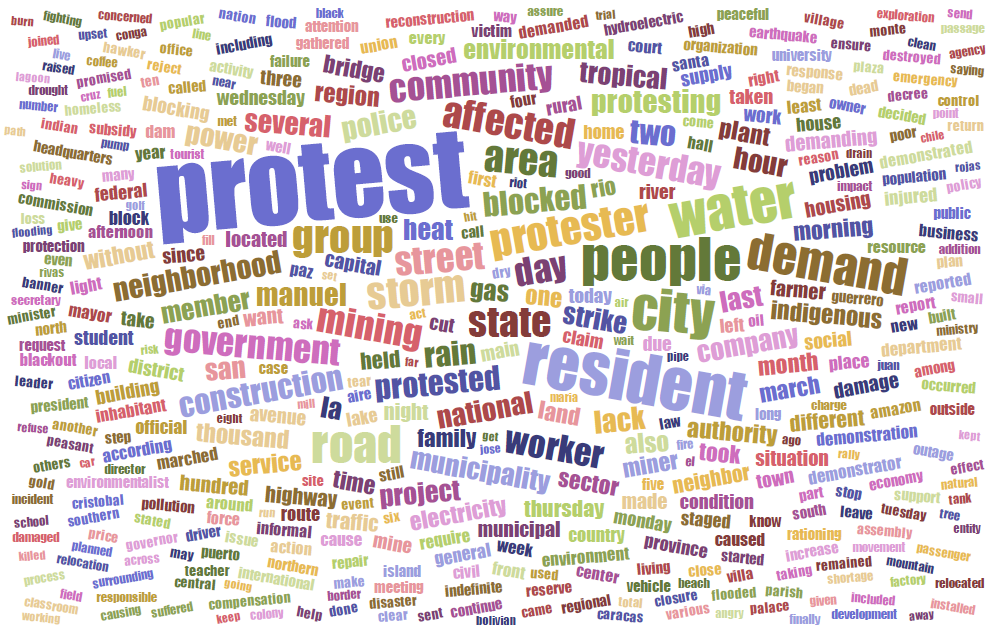
\includegraphics[width=.35\textwidth]{figures/Climate_word_cloud}}
\caption{Word cloud of all the climate related protests, from GSR descriptions.}
\label{wordcloud}
\end{figure}

In Figure~\ref{Mexico_disaster_timeseries}, the second red bar shows hurricane Odile 2014, belongs to category 3, whose track map can be seen in Figure~\ref{storm2014}. The interesting thing is, after hurricane Odile 2014, the more intense storm, there were not many related protests. Why? By checking Figure~\ref{Mexico-track-map}, we can see storm Manuel 2013 hit Mexico's mainland, which make it very destructive. While hurricane Odile 2014 caused lesser impacts on the Mexican mainland, even though it cross the state of Baja California Sur, however, it is the second smallest Mexican state by population. This can explain why storm 2013 lead to tremendous protests, while hurricane 2014 does not.

\paragraph{Brazil climate disasters}
Figure~\ref{Brazil_disaster_timeseries} shows Brazil climate disasters and climate protests relationship. The three yellow bar shows three drought events in Brazil, which caused drought related protests immediately. The drought in February 2012 hampered production, which arouse farmers protest. The heat wave in February in 2014, and drought in October 2014 results in water shortage, thus a series of protests against water shortage abrupt in Brazil. The biggest spike in June 2013 described protests against government's projects for the construction of hydroelectric plants in the Amazon region, which can be ascribed into environment category.


\paragraph{Venezuela climate disasters}
In Figure~\ref{Venezuela_disaster_timeseries}, the blue curve shows Venezuela climate related protests time series, and  vertical bars represent climate diasters. The rose bar represents sudden torrential rains in June 2013, caused a heightened risk of flooding and landslides in the densely populated communities on the outskirts of Caracas, and triggered a small portion of protests prevent flooding. The yellow bars denote drought disasters, of which the highest bar, represents a drought in May 2014, which triggered rationing of tap water in the capital, Caracas, where residents must form lines that last hours to fill jugs of water. This drought diaster lasted so long that related protests reached climax in September 2014.


\section*{5. Climate protests causality}

\subsection*{5.1 Word cloud}
Of the climate related protests, we are interested in what are the protesters demanding. To have a birds view of climate protests, we extract all the climate protest descriptions and plot the word cloud, as shows in Figure~\ref{wordcloud}. We can see words like `water', `storm', `mining', `rain', `construction', `power', `heat', `gas', `environment', `electricity', and other weather, environment related keywords are dominant, which gives us a general idea of what protesters are demanding.

\begin{figure}[t]
\centerline
{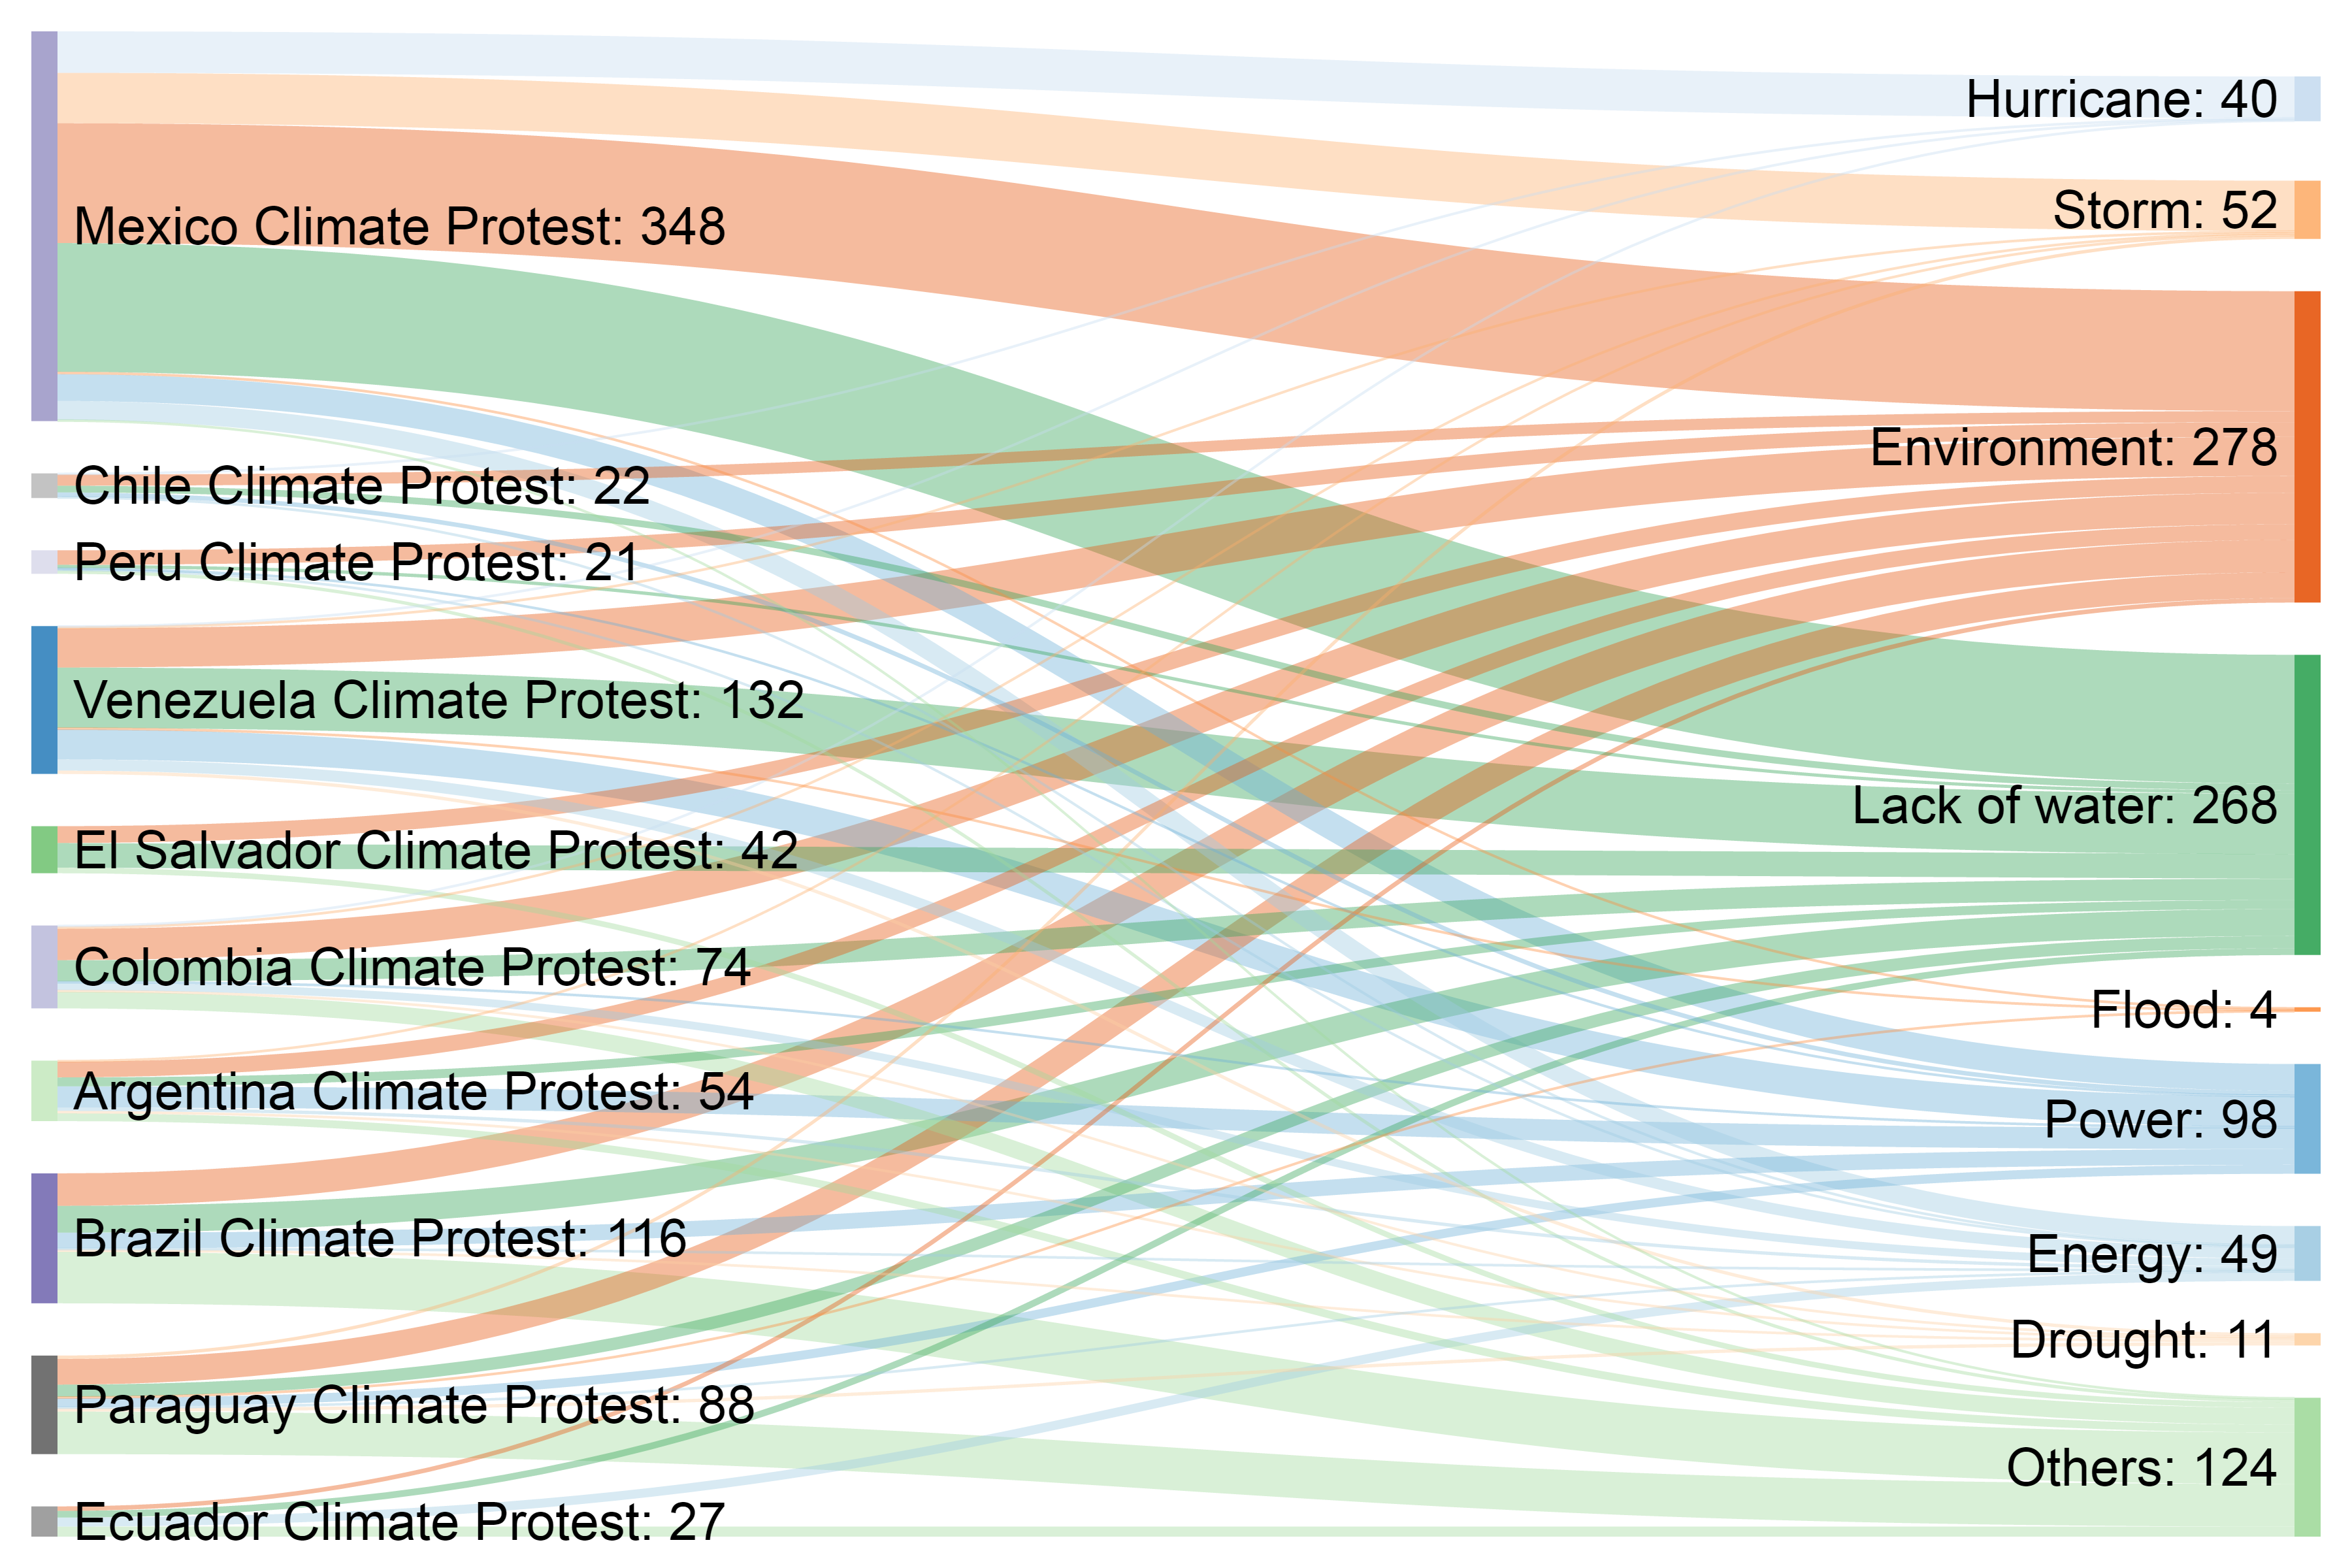
\includegraphics[width=.4\textwidth]{figures/causality1}}
\caption{Climate protest causality diagram. Left bar shows ten countries' climate protest numbers, and right bar shows nine climate event categories which cause climate protests.}
\label{causality}
\end{figure}

\subsection*{5.2 Climate protests proportion}
However, how is the proportion of each protest category, is still unclear. We build a classifier to categorize the climate protest types, which generally falls into nine categories. As can be seen in Figure~\ref{causality}, the most dominant two categories are environment concern and lack of water. After that, the third commonest reason is about power, blackout. Also, extreme weathers like storm, hurricane, drought also accounts a considerable portion. The interesting thing is, each country has its own distinguishing protest features. In Mexico, the most notable protest reasons are lack of water, environment concern, storm and hurricane. In Venezuela, apart from lack of water, environment problem, the dominant reasons are about blackout and energy issue. In Peru, more than half of climate protests are demanding mining project, which is related with environment concern. While in Argentina, 35\% events protest against blackout issue.


\begin{figure}[ht]
	\centering
	\subfigure[Mexico]{
		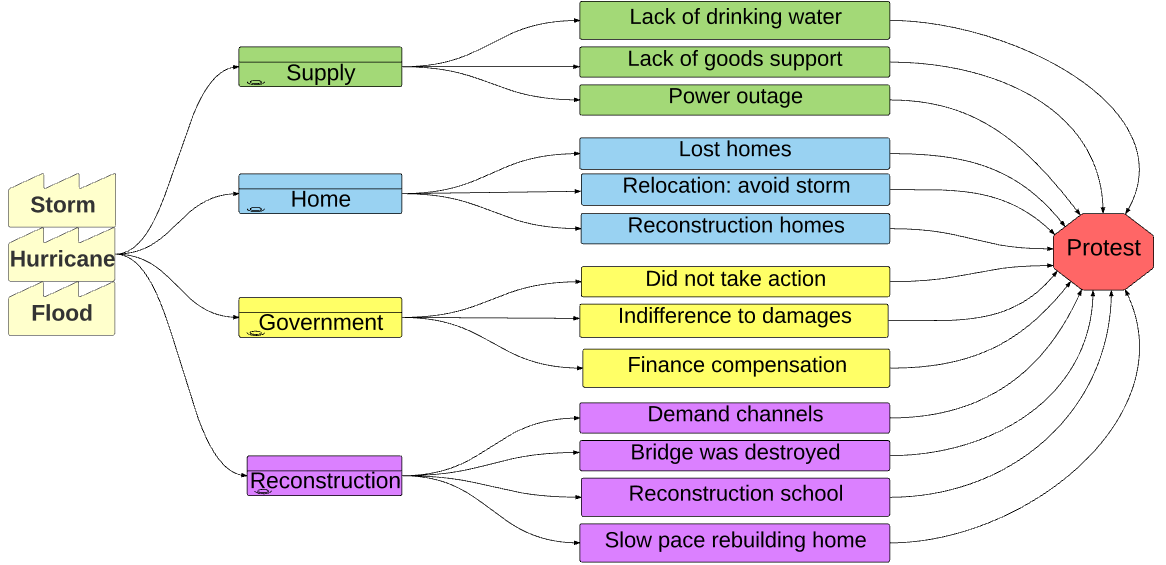
\includegraphics[width=3.2in] {figures/Mexico-diagram2}
		\label{Mexico_causality}
	}
	\subfigure[Brazil]{
		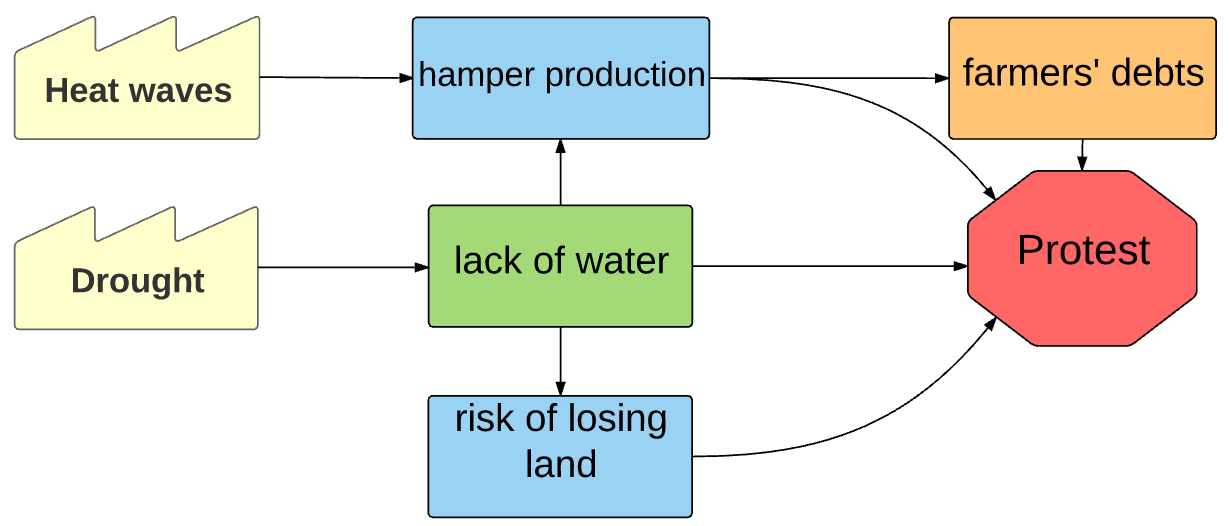
\includegraphics[width=1.55in, height=0.7in] {figures/Brazil-diagram}
		\label{Brazil_causality}
	}
    \subfigure[Venezuela]{
		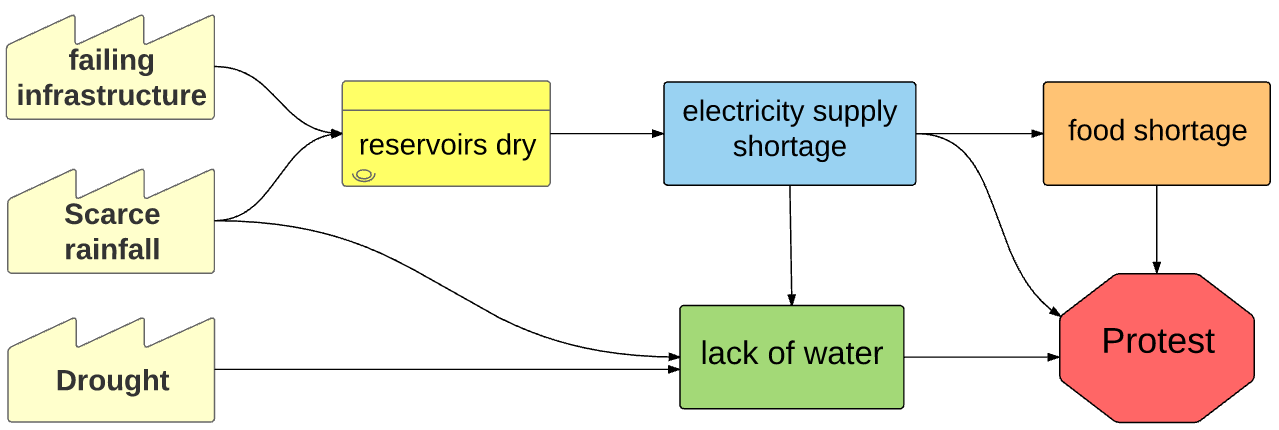
\includegraphics[width=1.55in, height=0.7in] {figures/Venezuela-diagram2}
		\label{Venezuela_causality}
    }
	\caption{Climate protest causality diagram}
\label{three-causality}
\end{figure}




\begin{figure*}[ht]
	\centering
	\subfigure[Brazil]{
		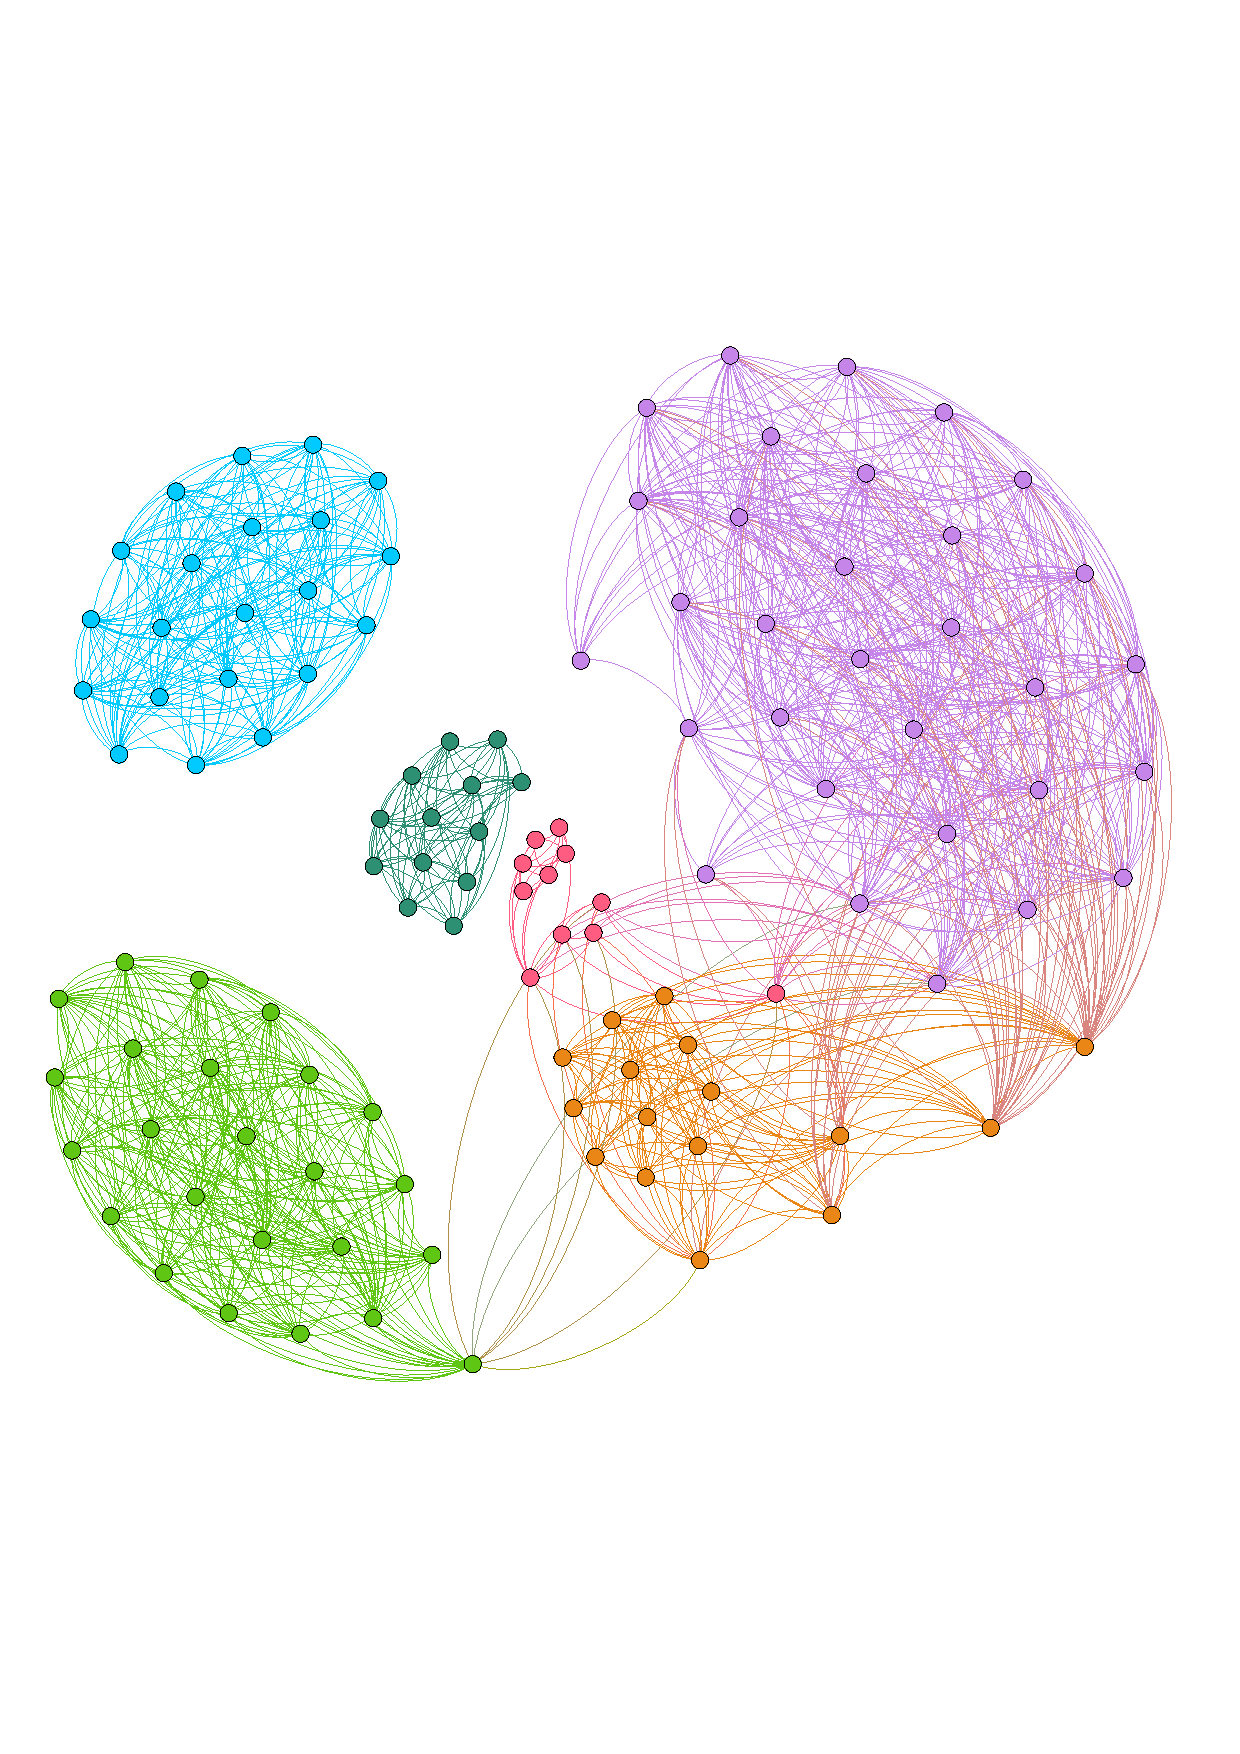
\includegraphics[width=2in, height=1.4in] {figures/Brazil_cluster}
		\label{Brazil_cluster}
	}
    \subfigure[Mexico]{
		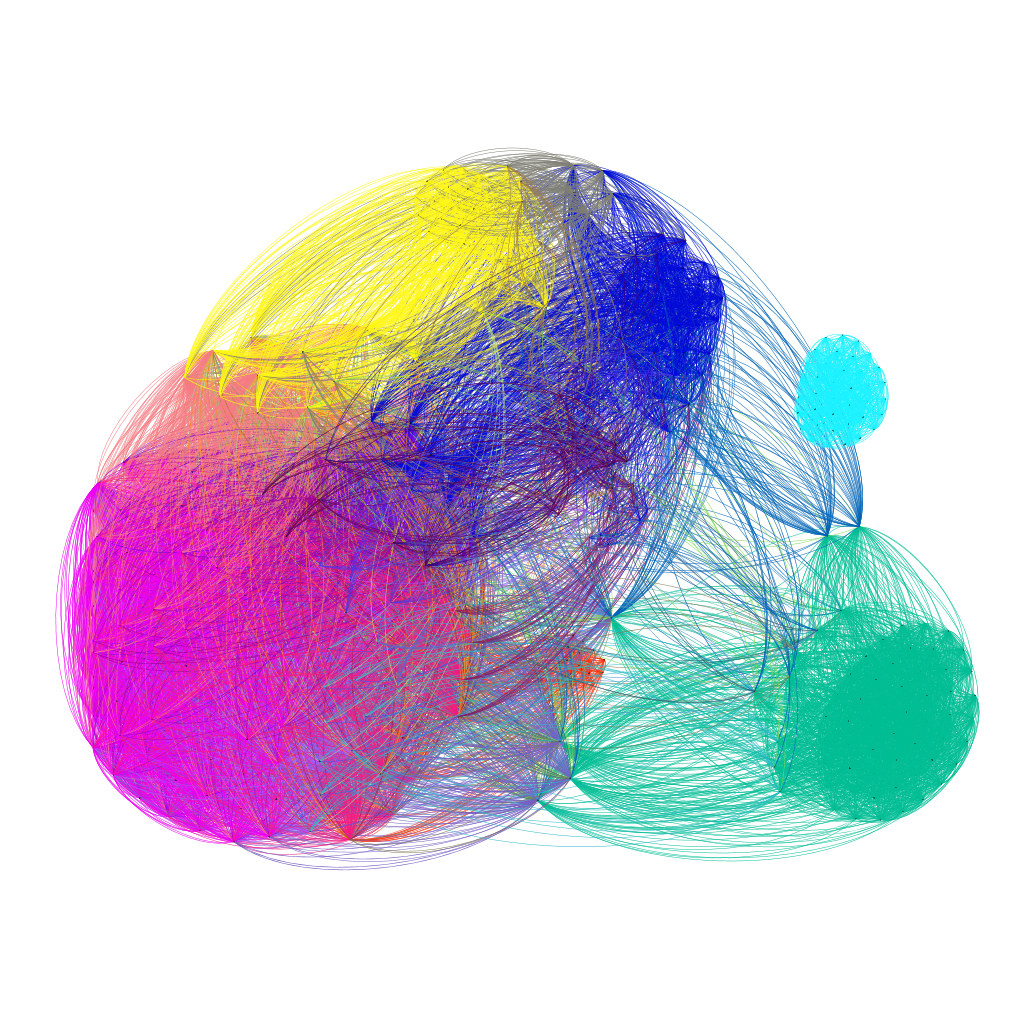
\includegraphics[width=2in, height=1.4in] {figures/Mexico_cluster1}
		\label{Mexico_cluster}
    }
	\subfigure[Venezuela]{
		\includegraphics[width=2in, height=1.4in] {figures/venezuela-cluster2}
		\label{Venezuela_cluster}
	}
	\caption{Climate protest clustering results}
\label{clusters}
\end{figure*}


\subsection*{5.3 Climate protests causality analysis}
More importantly, we intend to figure out the protests causality, how does the climate events involve into protests. The causality analysis is based on three steps, as described following.

a. Text enrichment.
Messages with textual content (Tweets, Newsfeeds, Blog postings, etc.) are subjected to shallow linguistic processing prior to analysis. Applying BASIS technologies' Rosette Language Processing (RLP) tools, the language of the text is identified, the natural language content is tokenized and lemmatized and the named entities identified and classified. Finally, messages are geocoded with a specification of the location (city, state, country), being talked about in the message.

b. Knowledge graph construction.
In the scope of this study, an entity network is a graph $G(E, R)$ where entities $E = {e_1,
. . ., e_n}$ can be linked to one another through relationships $R = {r_1, . . ., r_n}$ defined by conceptual interactions, and thus called a knowledge graph. knowledge graphs are used to represent its logic based on semantic networks.
How to represent knowledge and extract entities and their relationship from text?
The general extraction patterns rule is Noun Phrase - Verb Phrase - Noun Phrase. We can also employ multilingual rules for phrase patterns learnt using association mining based on collocations. Using an open source, GraphDb (Neo4j) to store and query knowledge triples.
%Neo4j is a very robust, scalable solution for Knowledge representation, which provides an expressive query language : CYPHER, and a framework for implementing graph theoretic search algorithms.
The general scheme is Subject - Predicate - Object. Subject is a concept, which can be person, organization, location, event, noun phrase; Predicate can be either a verb action or (predefined) relation type; Object can be either a concept or (some) value. With all the enriched articles as input, since their named entities and verb phrases being identified and classified, the system can automatically extract the structural knowledge and load them into Graph database. It worths to note the entities may evolve along space and time.

c. Causality query.
With a complete knowledge database, we are going to poses domain specific questions, for example, who are the main players in the article? what are the reasons for the protest? To such questions like that, we are seeking causal (base) relations between concepts. Specifically, we are interested in entities to be storm, hurricane, heat, draught, etc,, climate related keywords. By matching the object or subject with climate related keywords, and predicate to be causality relationship like result of, cause by, lead to, blamed, accused of, demanding, against, request, we can locate and further identify the event-specific descriptors, get the relations between concepts (players and protest keywords) or relations of base type - temporal, change state, explicit facts.

%match (a)-[relations]-(b) where a.name =~ '.*climate.*', and a.relations =~ '.*cuase.*'  return a, relations, b. We are interested in relations like 'cause', 'demanding', 'against', 'request', and so on.

For some severe and dominant climate events, such as storm, hurricane, flood, and drought events, we use the knowledge graph to identify their evolution pattern, thus from climate disasters, how does it evolve into armed conflicts? As shown in Figure~\ref{three-causality}, we illustrate storm caused protests demands in Mexico, blackout caused protest demands in Venezuela, and drought caused protest demands in Brazil.


\paragraph{6. Climate protest pattern}
According to the protest content, we cluster each country's protests type. Based on protest descriptions, we calculate two descriptions text similarity, and assign weight between the two protest IDs. Specially, we pay special attention to the protest themes or protest demands, if two descriptions have the same protest demanding, they will have high weight, otherwise, if their protest demanding are different, their connection weight tends to be 0. In this way, we build a weighted undirected network $G(V, E, W)$, with each protest as node $V$, and their connection as edge $E$, their weight as $W$. If the weight between two nodes is 0, their will be no edge. We employ Louvain method~\cite{blondel2008fast} to split the network into several clusters.


For Brazil's climate protests, as can be seen in Figure~\ref{Brazil_cluster}, the purple cluster which represents land ownership accounts the most part, 26.7\%, the green cluster which denotes lack of water accounts 20.7\%, farmers cluster accounts 13.8\%. The interesting thing is land and farmers clusters are closely coherent. Amazon rainforest is another striking protest which accounts for 11.3\%.

For Mexico's climate protests, as shown in Figure~\ref{Mexico_cluster}, the rose red cluster which denotes lack of water is the most dominant protest, accounts for 20.5\%, the green cluster tropical storm is the second largest protest type, 19.0\%, the dark blue cluster construction accounts for 17\%, and the yellow cluster land accounts for 11.8\%. The interesting thing is, water protest is intertwined with environment protest and power protest, land protest is closely related with farmers, while construction cluster is coherent with baby blue cluster (2.6\%) which denotes homes.


For Venezuela's climate protests, as can be seen in Figure~\ref{Venezuela_cluster}, the yellow cluster which represents lack of water protests accounts for 55.8\%, the green cluster which denotes power outage accounts for 22.1\%, and the blue cluster which stands for gas shortage accounts for 5\%, the purple cluster shows the rest climate protest portion, which include food shortage, medicine shortage, water tank robbery behavior, etc..



\begin{figure}[t]
	\centering
	\subfigure[Mexico]{
		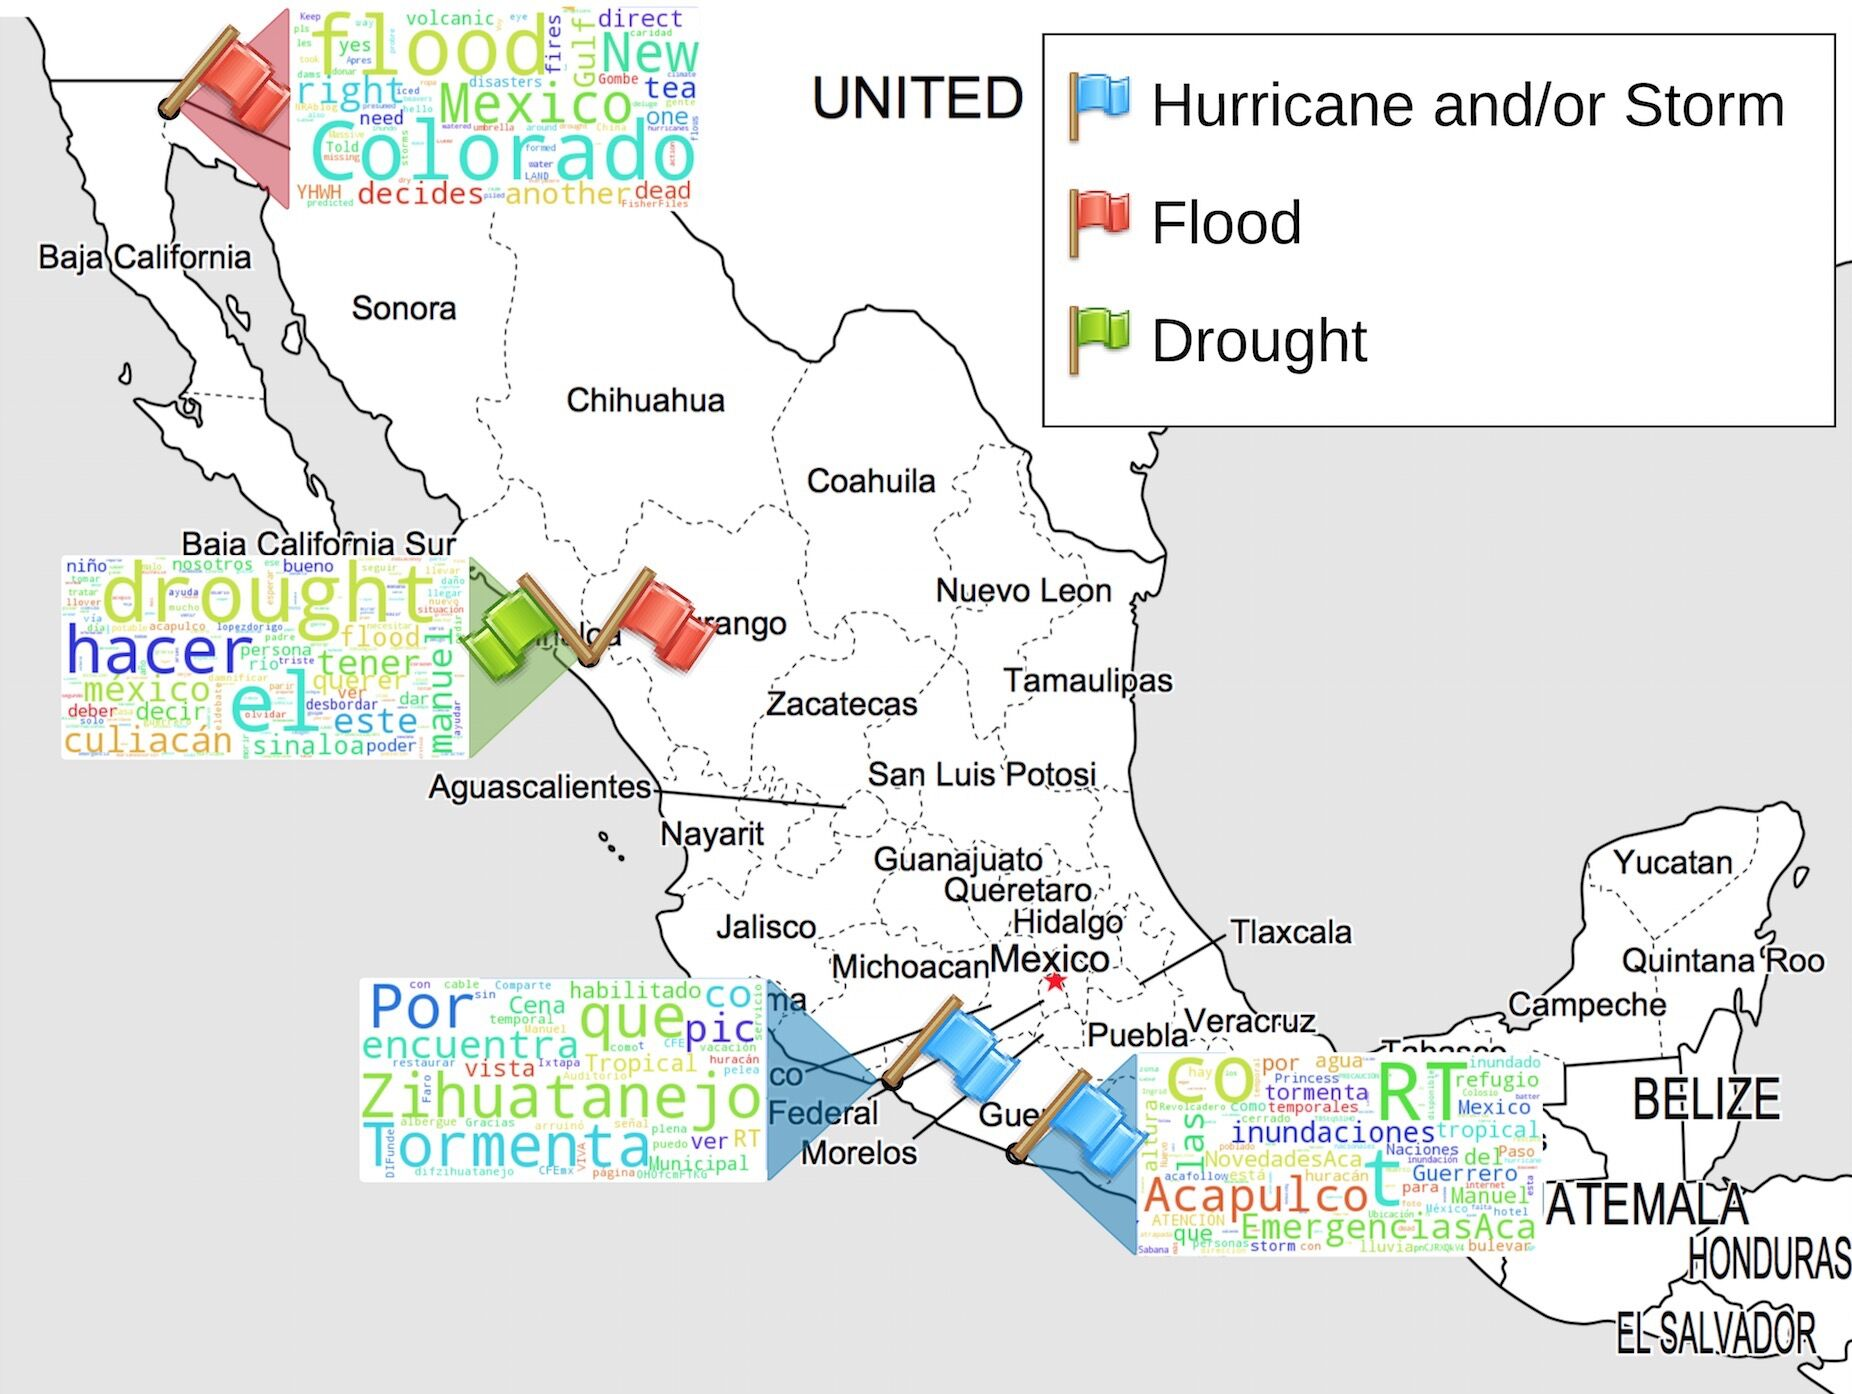
\includegraphics[width=1.6in, height=1.3in] {figures/Mexico-events}
		\label{Mexico-events}
	}
	\subfigure[Brazil]{
		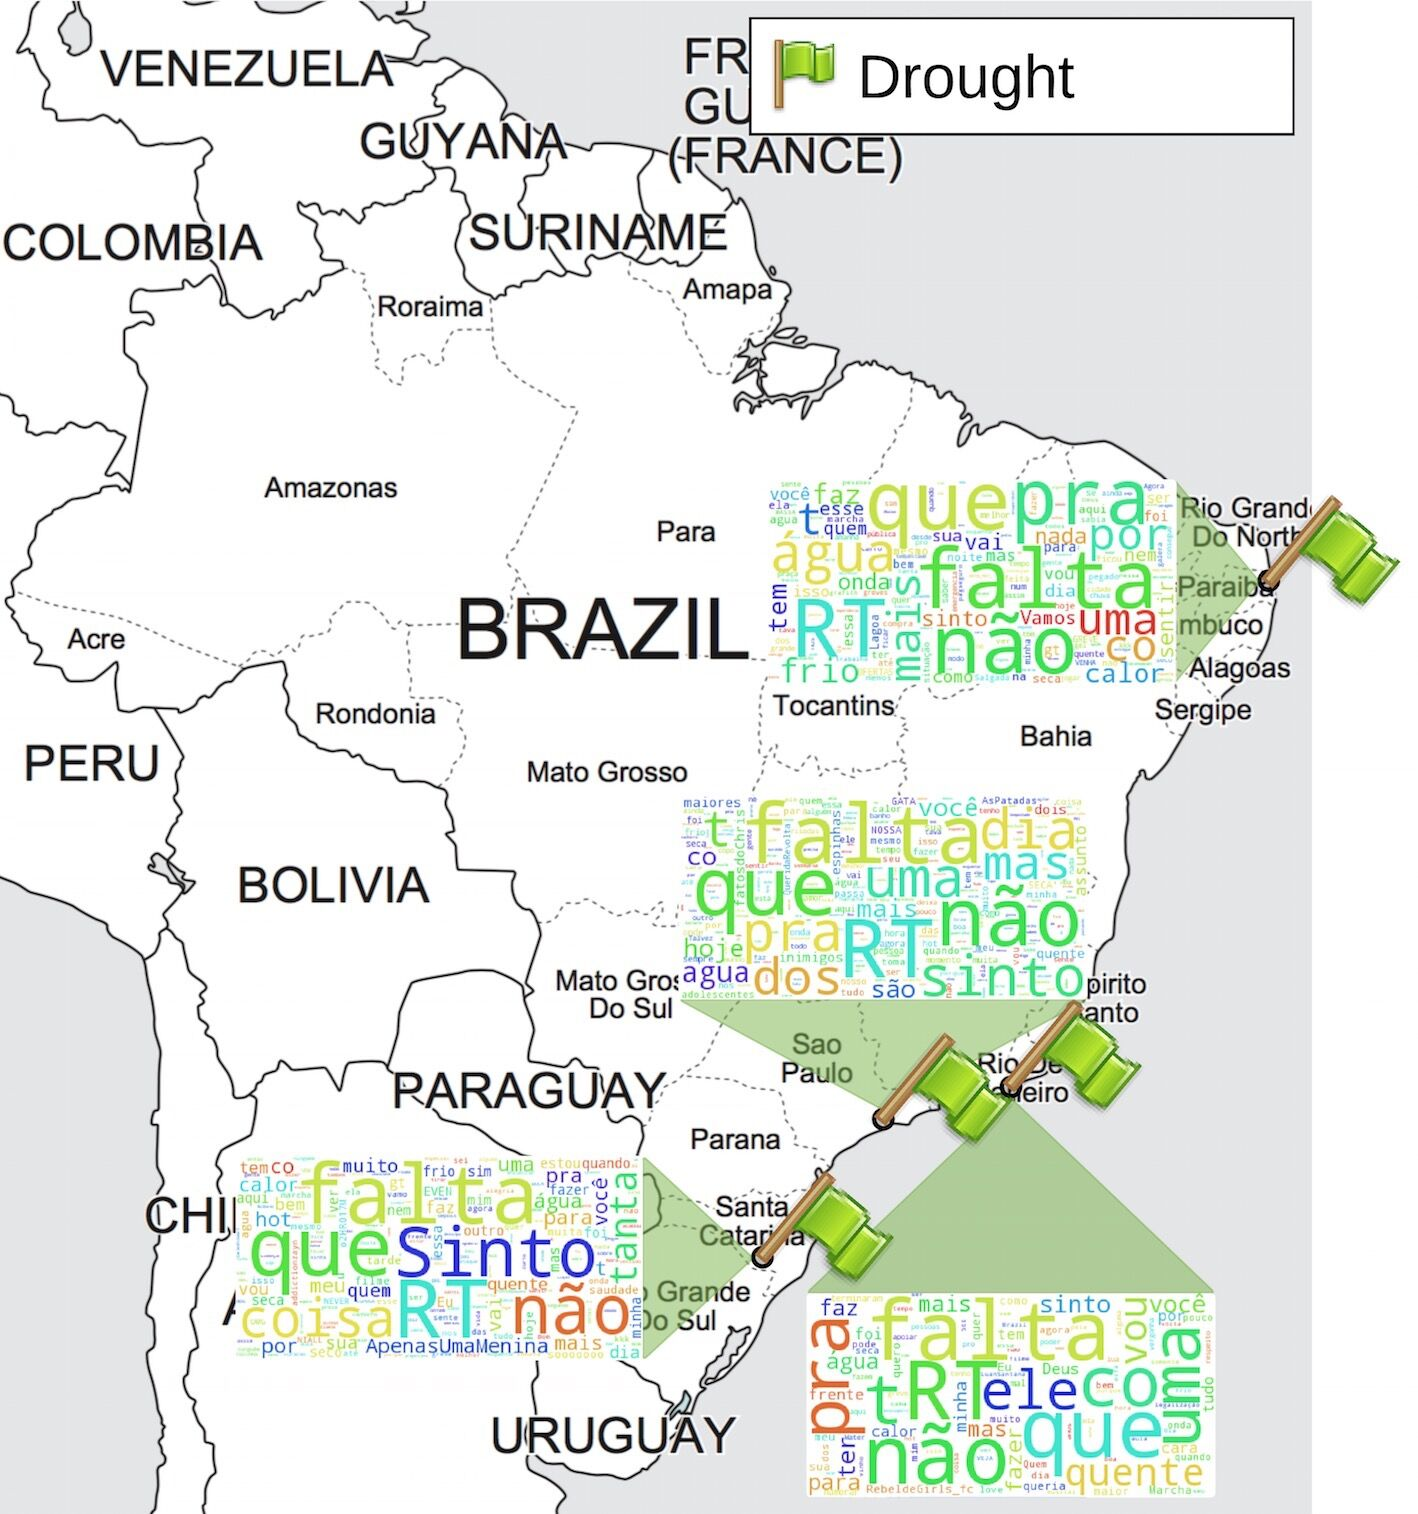
\includegraphics[width=1.45in, height=1.3in] {figures/Brazil-events}
		\label{Brazil-events}
	}
	\caption{Climate protest events in Mexico, Sept 2013 and Brazil, May 2012. Different flag represents different climate disasters. The adjacent world cloud shows Twitter discussion as per that event. }
\label{Twitter-events}
\end{figure}

\paragraph{7. Climate protests in Twitter}
We are also interested in climate events influence on social media, such as Twitter. Using keywords list we are able to filter tweets, then cluster tweets into different partitions based on similarity among tweets using distance function, taking tweets content, geolocation and other features into consideration. Each partition includes similar tweets stand for a specific event. As shown in Figure~\ref{Mexico-events}, there are three distinct extreme weather event type in Mexico in different locations, the word cloud shows discussion on Twitter as per that event.


%\begin{figure}[ht]
%\centerline
%{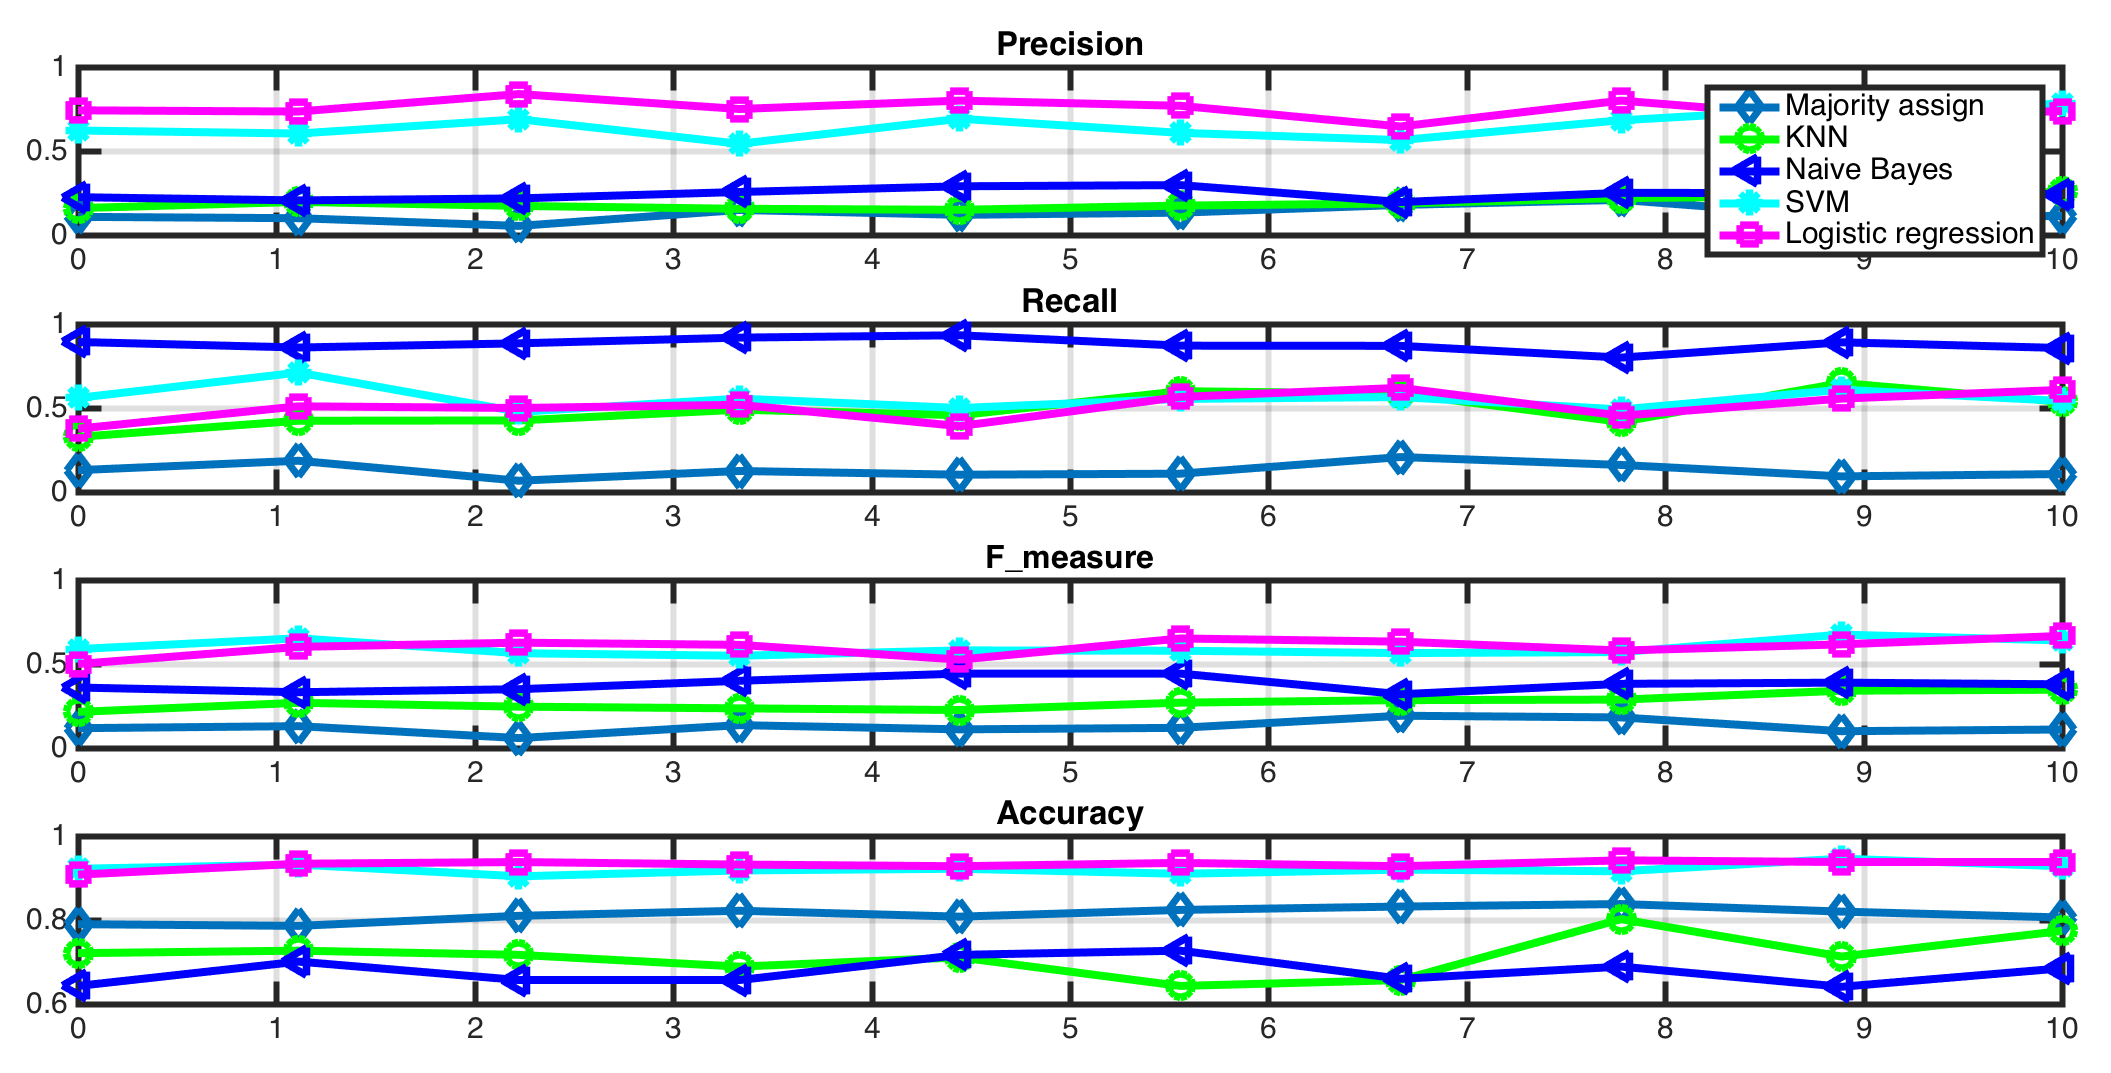
\includegraphics[width = 3in, height=1.5in]{figures/resultsComp1}}
%\caption{Classification methods comparison.}
%\label{resultsComp}
%\end{figure}


\section*{Discussion}
\matmethods{
%Please describe your materials and methods here. This can be more than one paragraph, and may contain subsections and equations as required. Authors should include a statement in the methods section describing how readers will be able to access the data in the paper.
\paragraph{Dataset: GSR}
Using human analysts, MITRE organizes a gold standard report (GSR) of protests by surveying newspapers for reportings of civil unrest. The GSR includes many features, as shown in Figure~\ref{GSR}, such as protest location, event date, protest type, status, crowd size, headline, date, population, protest description, first reported links, etc.. The description feature is brief description of the protest, generally, it tells us who, where, why and when protest. As Figure~\ref{GSR} shows, the protest description is `small farmers want the bank to forgive their debts due to the drought, which has hampered production'.

\begin{figure}[th]
\centerline
{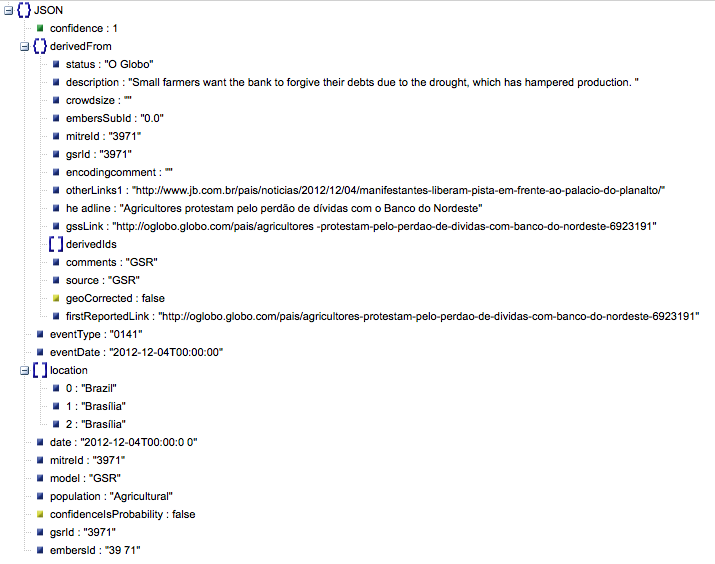
\includegraphics[width = 2.5in]{figures/gsr_event_json.png}}
\caption{Gold standard report (GSR) format.}
\label{GSR}
\end{figure}

\paragraph{Climate protest classifier}
a. Method. From GSR events, we devised a climate protest classifier to identify the climate related protest events automatically. The classifier is built based on logistic regression model. With input of GSR descriptions, we aim to train a classifier which can label a protest description as climate related or not. The GSR includes many potential important features, such as status, description, crowd size, headline, event Type, event Date, location, date, population etc. The description feature is brief description of the events, which plays a dominant role in the entire dataset. In order to adopt logistic regression on GSR dataset, we need to vectorize text data in the dataset. First of all, we construct a word corpus which includes every word $x_i$ shown in the training dataset (including non-words). We accept non-words because most coinages come from Internet and some of them might be important for the events. As we accept non-words, the corpus might be large than our corpus vocabulary. The word corpus is composed with $[x_1, x_2, ..., x_i, ..., x_N]$.
Second, take each GSR description as a vector, we assign values to each vector, if $x_i$ appeared in GSR record, the corresponding value will be assigned as 1, otherwise 0. In this way, every GSR record being converted to a corresponding vector based on the corpus. Third, set climate protest as $Y=1$, non-climate protest as $Y=0$, the weight for each term $x_i$ as $k_i$, then $Y_j = \sum_{i=1}^{N} k_i x_i $. By training process, we calculate the weight $k_i$ for each term $x_i$. The last step is test. Given a new GSR description, the probability of classification is:
$$P(Y = 0| X)= \frac{1}{1+exp( {\sum_{i=1}^{N} k_ix_i})}$$
$$P(Y = 1| X)= \frac{exp( {\sum_{i=1}^{N} k_ix_i})}{1+exp( {\sum_{i=1}^{N} k_ix_i})}$$


b. Evaluation. We manually labelled 1700 GSR protest records as climate or non-climate protests. Using 70\% dataset as training, and the rest 30\% as test. To ensure we have a trustworthy classification results, we evaluate the performance carefully by cross evaluation. The evaluation criteria are precision (positive predictive value), recall (true positive rate), F-measure (a measure that combines precision and recall) and accuracy (the proportion of true results both true positives and true negatives among the total number of cases examined). We compare with four well-known classification methods: majority assign, K-nearest neighbor, Naive Bayes, and weighted support vector machine (SVM). Since the climate events account for a small portion of all the events, which make it an unbalanced classification problem, so we change the traditional support vector machine into weighted SVM, by adding more importance to the climate portest events (we set the class weight to be 100). From Table~\ref{table:comparision}, we prove logistic regression method outperforms other methods uniformly.

\begin{table}[!ht]
\small
\caption{Classification methods comparison.}
\vspace{0.5em}
\centering
\begin{tabular}{|c | c | c | c | c |}
\hline
 & \textbf{Precision} & \textbf{Recall} & \textbf{F\_ measure} & \textbf{Accuracy}  \\ [1ex]
\hline
Majority assign   &  0.1274  &  0.1289 &  0.1258 &  0.8136  \\[1ex]
\hline
KNN &  0.1906  & 0.4913 &  0.2723 &  0.7154  \\[1ex]
\hline
Naive Bayes &  0.2432 & 0.8779 &  0.3798 &  0.6777  \\[1ex]
\hline
Weighted SVM &  0.6543 &  0.5565 & 0.5966 &  0.9218  \\[1ex]
\hline
Logisitic Regression & 0.7513 &  0.5102 &  \textbf{0.6018}&  \textbf{0.9322}  \\[1ex]
\hline
\end{tabular}
\label{table:comparision}
\end{table}


\paragraph{Conclusion} We build a climate protest classifier based on the logistic linear regression model, which achieves the best performance comparing with other classical classifiers. We analysis the climate related protest both temporally and geographically. Further more, we investigate the climate protest causalities, and show that the shortage of water and electricity tops the climate protests. Finally, we also demonstrate the climate protests patterns and its influence on twitter.

}

\showmatmethods % Display the Materials and Methods section


\acknow{Supported by the Intelligence Advanced Research Projects Activity (IARPA) via DoI/NBC contract number D12PC000337, the US Government is authorized to reproduce and distribute
reprints of this work for Governmental purposes notwithstanding any copyright annotation thereon. Disclaimer: The views and conclusions contained herein are those of the authors and should not be interpreted as necessarily representing the official policies or endorsements, either expressed or implied, of IARPA, DoI/NBC, or the US Government.}

\showacknow % Display the acknowledgments section

% \pnasbreak splits and balances the columns before the references.
% If you see unexpected formatting errors, try commenting out this line
% as it can run into problems with floats and footnotes on the final page.
\pnasbreak

% Bibliography
\bibliography{pnas-sample}



\end{document}

%\begin{figure}[ht]
%\centerline
%{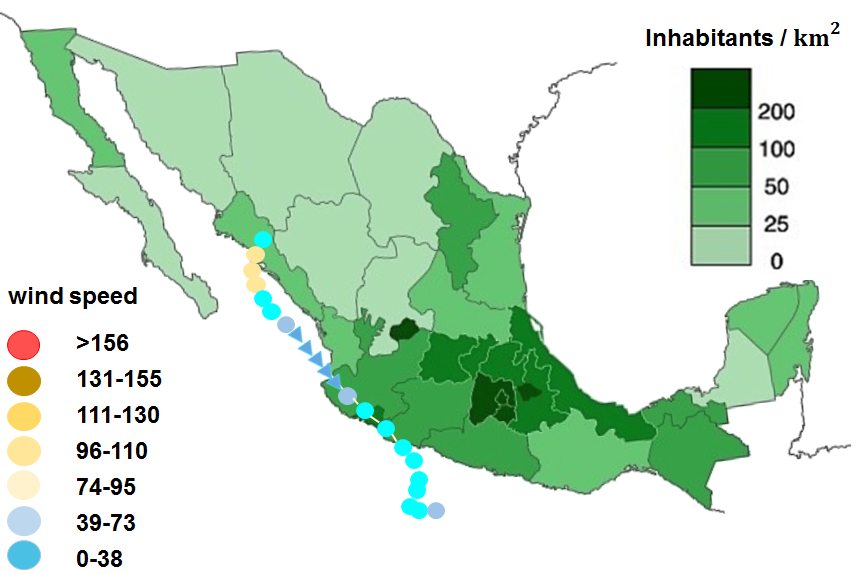
\includegraphics[width=.4\textwidth]{figures/Mexico-2013-Manuel}}
%\caption{Track map of Tropical Storm Manuel of the 2013 Pacific hurricane season. The points show the location of the storm at 6 hour intervals. The colour represents the storm's maximum sustained wind speeds as classified in the Saffir Simpson hurricane wind scale, and the shape of the data points represent the nature of the storm. The map shows population density of all Mexico's 32 states.}
%\label{storm2013}
%\end{figure}
%
%
%\begin{figure}[ht]
%\centerline
%{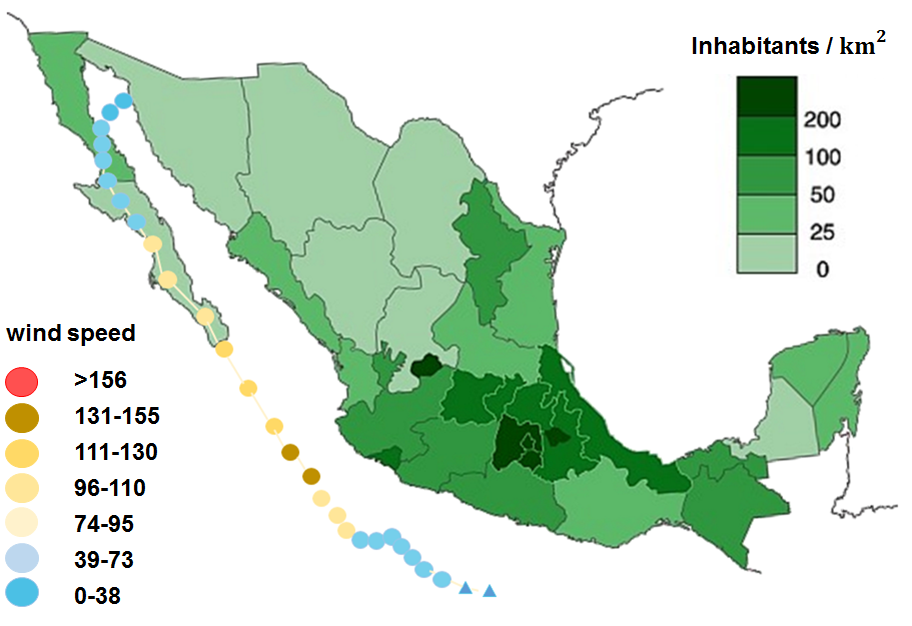
\includegraphics[width=.4\textwidth]{figures/Mexico_2014_Odile1}}
%\caption{Track map of Hurricane Odile of the 2014 Pacific hurricane season. The points show the location of the storm at 6 hour intervals. The colour represents the storm's maximum sustained wind speeds as classified in the Saffir Simpson hurricane wind scale, and the shape of the data points represent the nature of the storm. The map shows population density of all Mexico's 32 states.}
%\label{storm2014}
%\end{figure}

%\begin{figure}[ht]
%	\centering
%	\subfigure[Climate]{
%		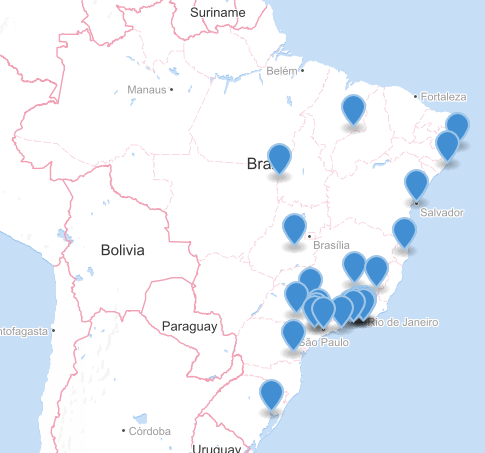
\includegraphics[width=1.4in] {figures/Brazil-climate-map}
%		\label{Brazil_climate}
%	}
%	\subfigure[Non-climate]{
%		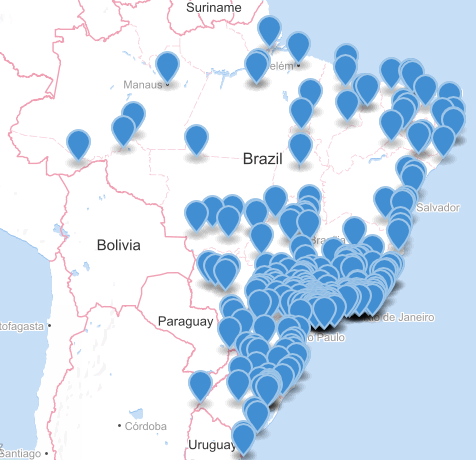
\includegraphics[width=1.4in] {figures/Brazil-non-climate-map}
%		\label{Brazil_non-climate}
%	}
%	\caption{Climate and non-climate protests in Brazil, from July 2012 to March, 2015.}
%\label{Brazil_two_maps}
%\end{figure}


%\begin{figure}[ht]
%	\centering
%	\subfigure[Climate]{
%		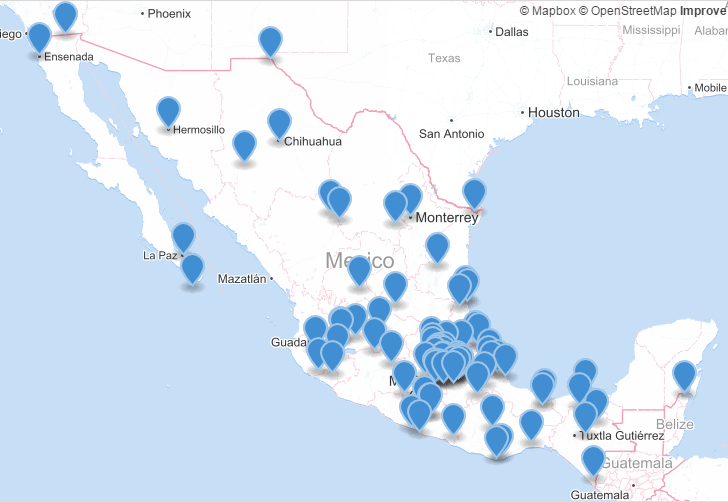
\includegraphics[width=1.5in] {figures/Mexico_climate}
%		\label{map_Mexico_climate}
%	}
%	\subfigure[Non-climate]{
%		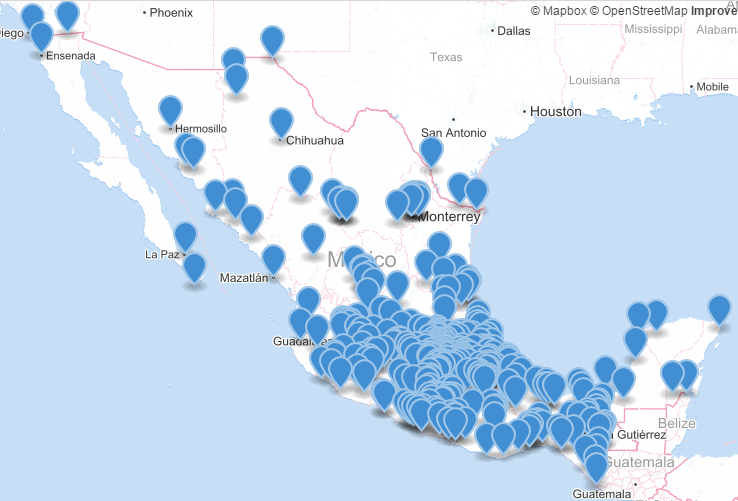
\includegraphics[width=1.5in] {figures/Mexico_non-climate}
%		\label{map_Mexico_non-climate}
%	}
%	\caption{Climate and non-climate protests in Mexico, from July 2012 to March, 2015. }
%\label{Mexico_map}
%\end{figure}



%\begin{figure}[ht]
%	\centering
%	\subfigure[Climate]{
%		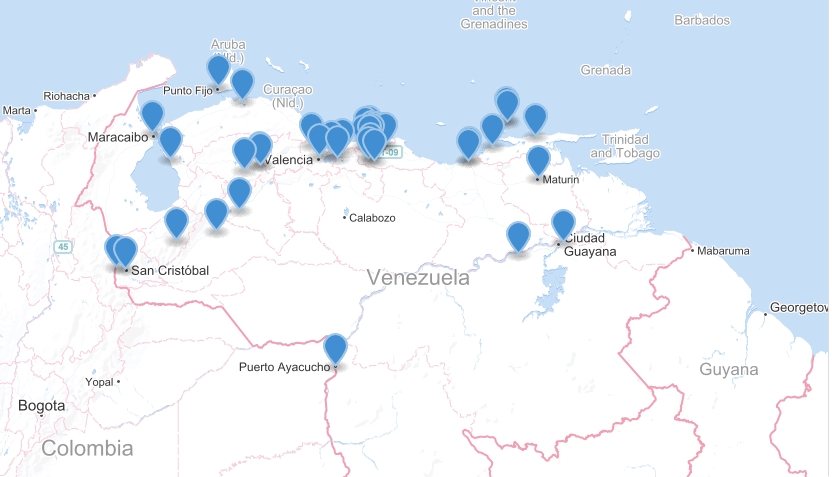
\includegraphics[width=1.5in] {figures/Venezuela-climate}
%		\label{map_Venezuela_climate}
%	}
%	\subfigure[Non-climate]{
%		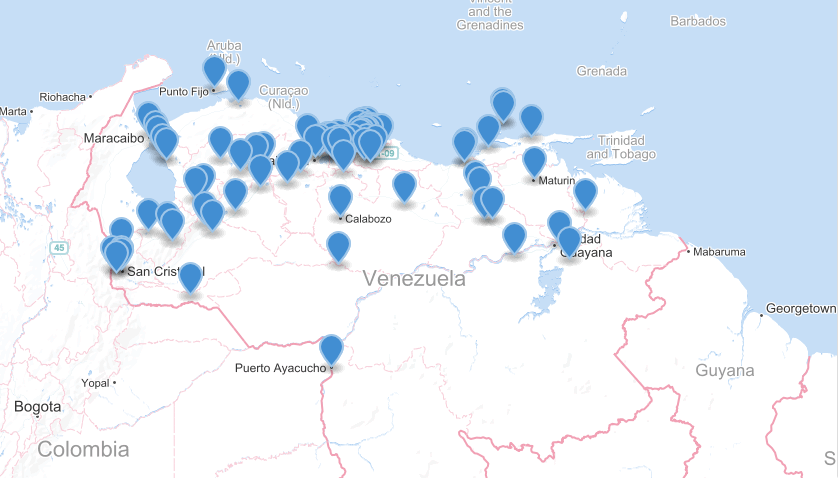
\includegraphics[width=1.5in] {figures/Venezuela-non-climate}
%		\label{map_Venezuela_non-climate}
%	}
%	\caption{Climate and non-climate protests in Venezuela, from July 2012 to March, 2015. }
%\label{Venezuela_map}
%\end{figure}



%\begin{figure}[ht]
%\centerline
%{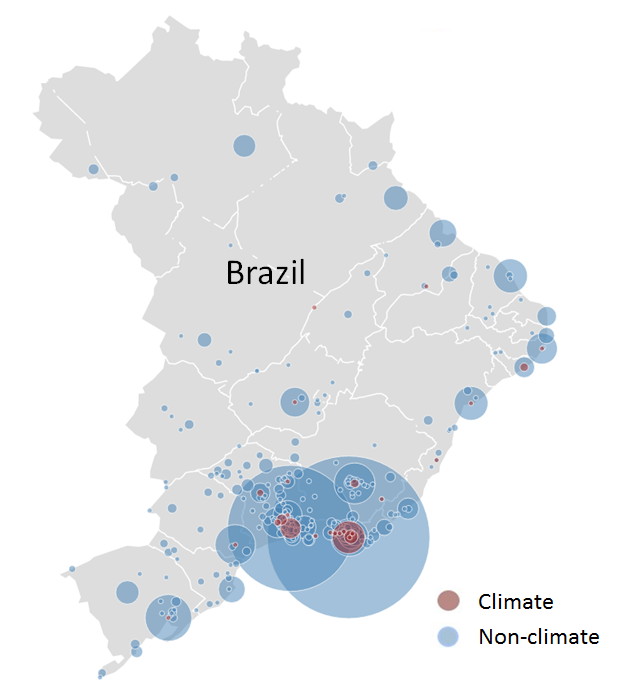
\includegraphics[width=.3\textwidth]{figures/Brazil}}
%\caption{Climate and non-climate protests in Brazil, from July 2012 to March, 2015. Red circle represents climate related protest events, and blue circle represents non-climate related protests. }
%\label{Brazil_map}
%\end{figure}
%
%
%\begin{figure}[ht]
%\centerline
%{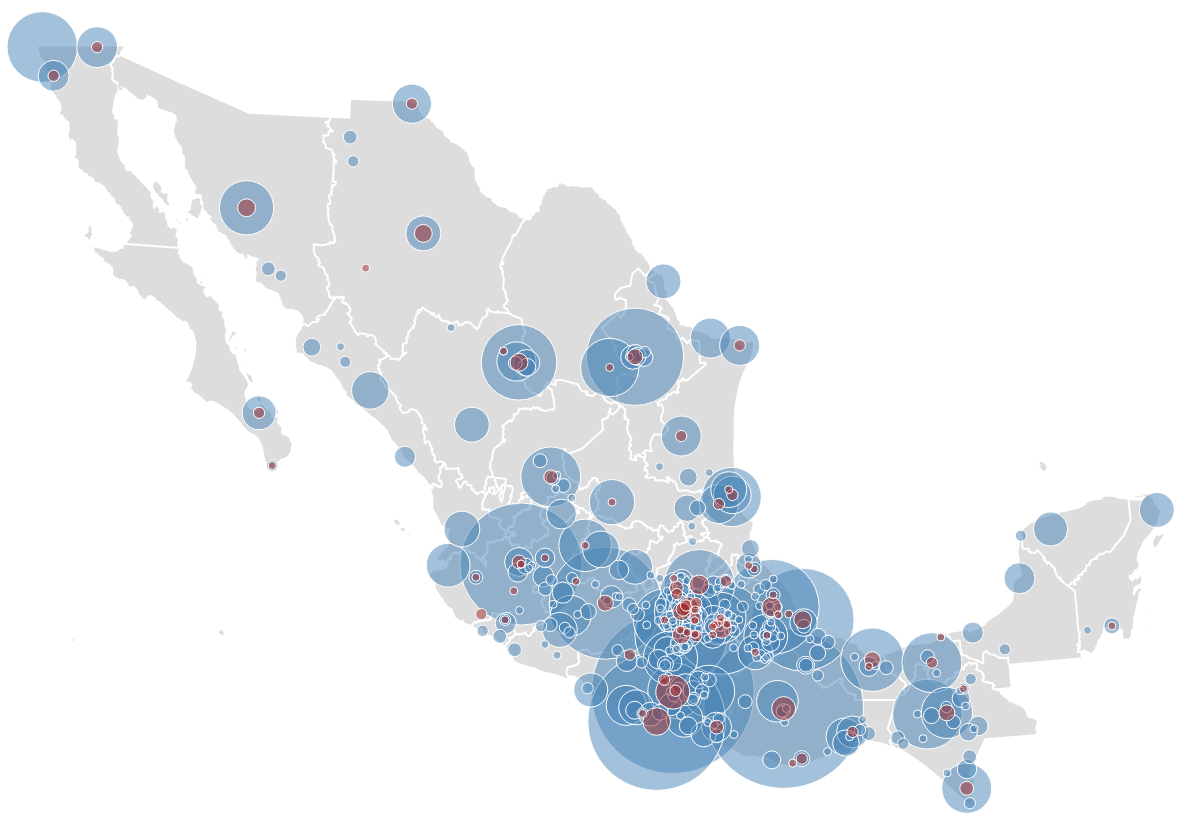
\includegraphics[width=.35\textwidth]{figures/Mexico_climate_non-climate}}
%\caption{Climate and non-climate protests in Mexico, from July 2012 to March, 2015. Red circle represents climate related protest events, and blue circle represents non-climate related protests. }
%\label{Mexico_map}
%\end{figure}
%
%
%\begin{figure}[ht]
%\centerline
%{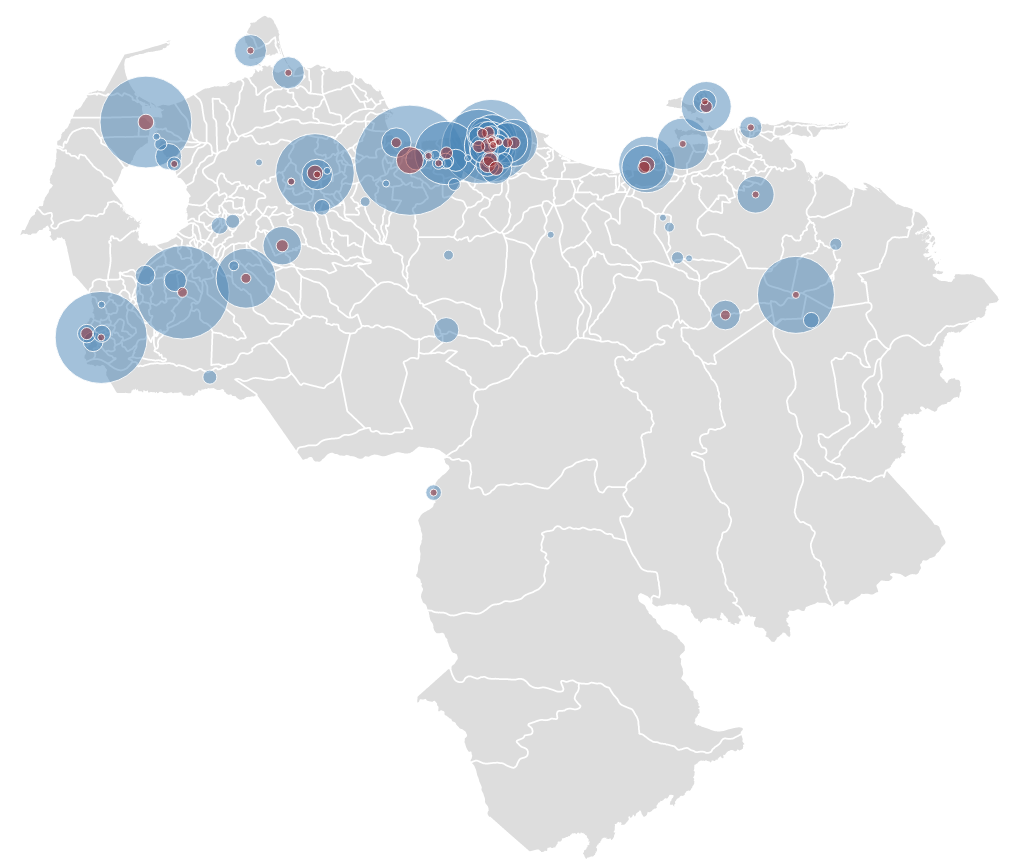
\includegraphics[width=.35\textwidth]{figures/Venezuela_climate_non-climate}}
%\caption{Climate and non-climate protests in Venezuela, from July 2012 to March, 2015. Red circle represents climate related protest events, and blue circle represents non-climate related protests. }
%\label{Venezuela_map}
%\end{figure}



%\begin{figure}[ht]
%\centerline
%{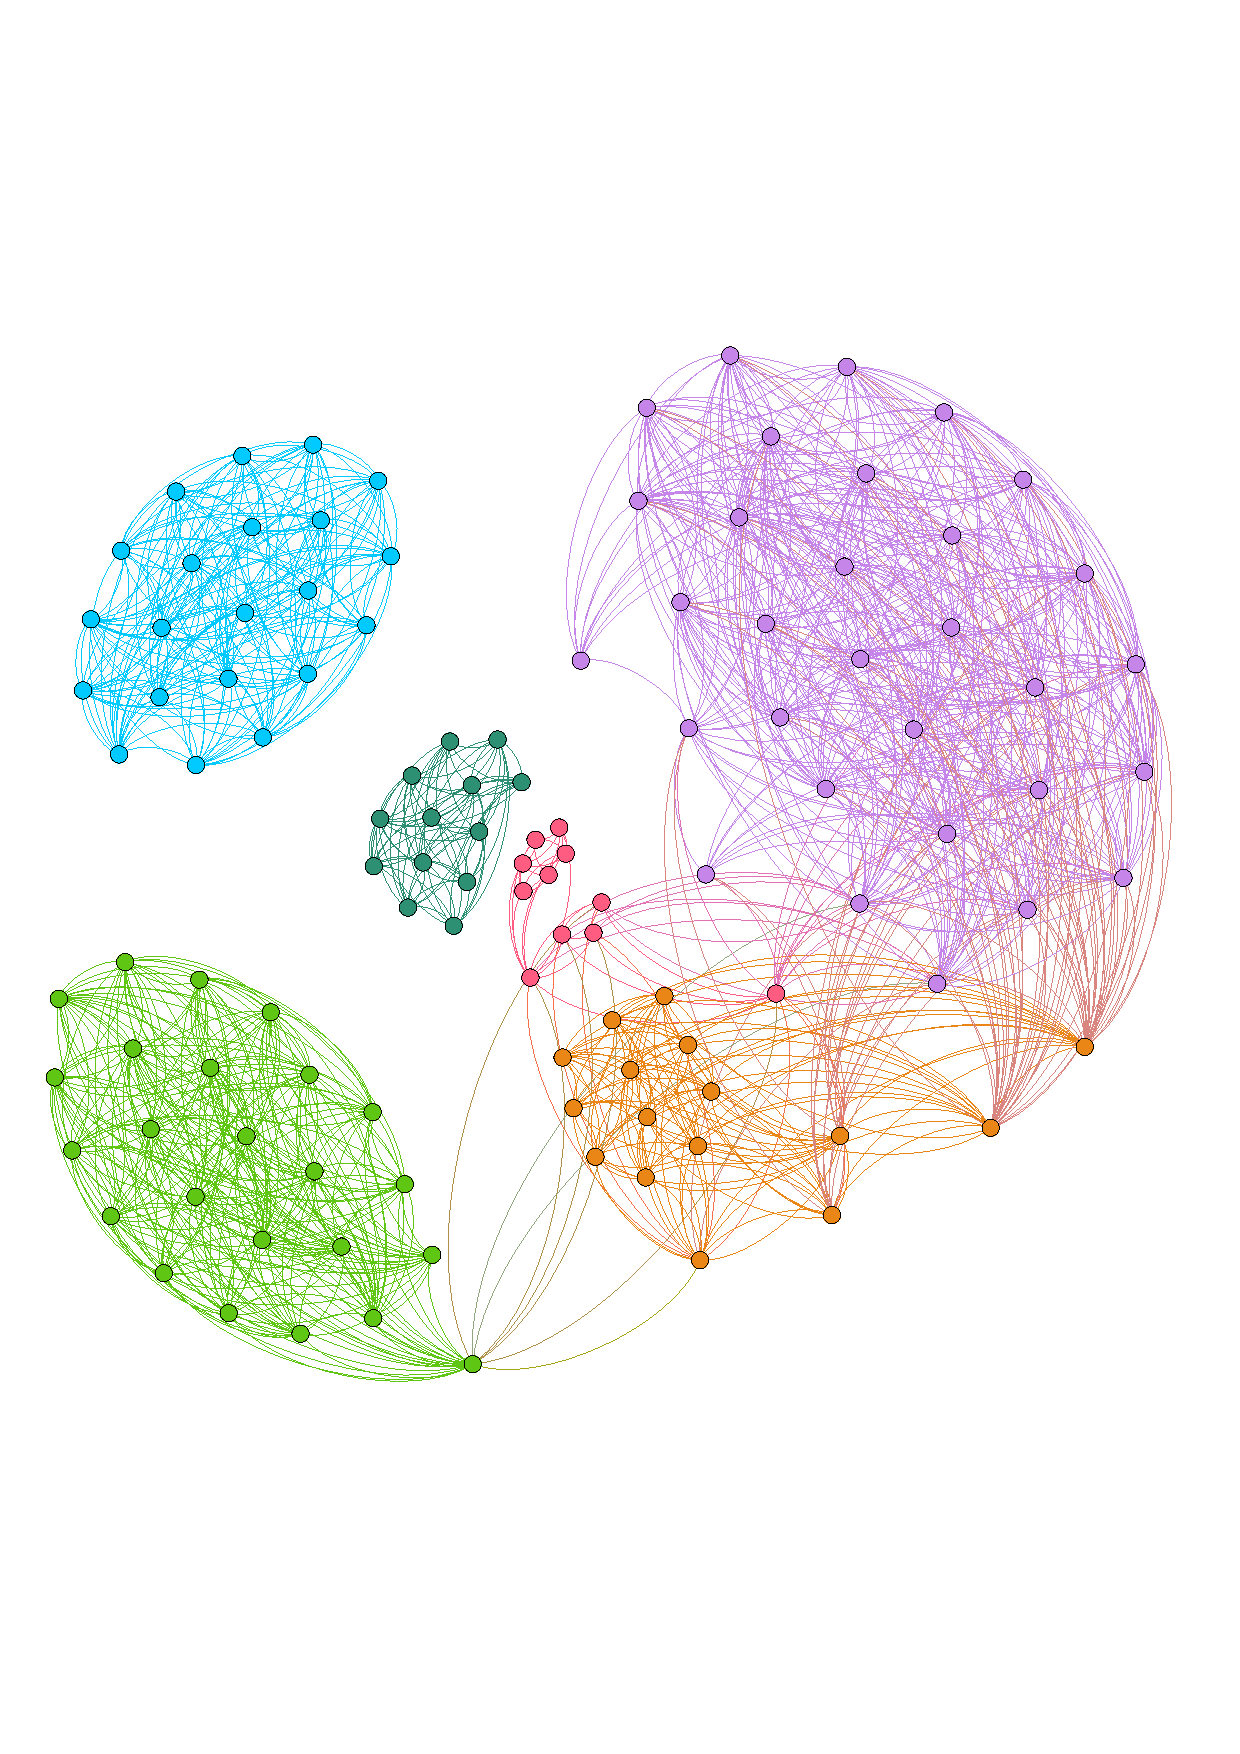
\includegraphics[width = 3.5in]{figures/Brazil_cluster}}
%\caption{Brazil protests clustering results.}
%\label{Brazil-cluster}
%\end{figure}
%
%\begin{figure}[ht]
%\centerline
%{\includegraphics[width = 3.5in]{figures/venezuela-cluster2}}
%\caption{Venezuela protests clustering results.}
%\label{Venezuela-cluster}
%\end{figure}
%
%
%\begin{figure}[ht]
%\centerline
%{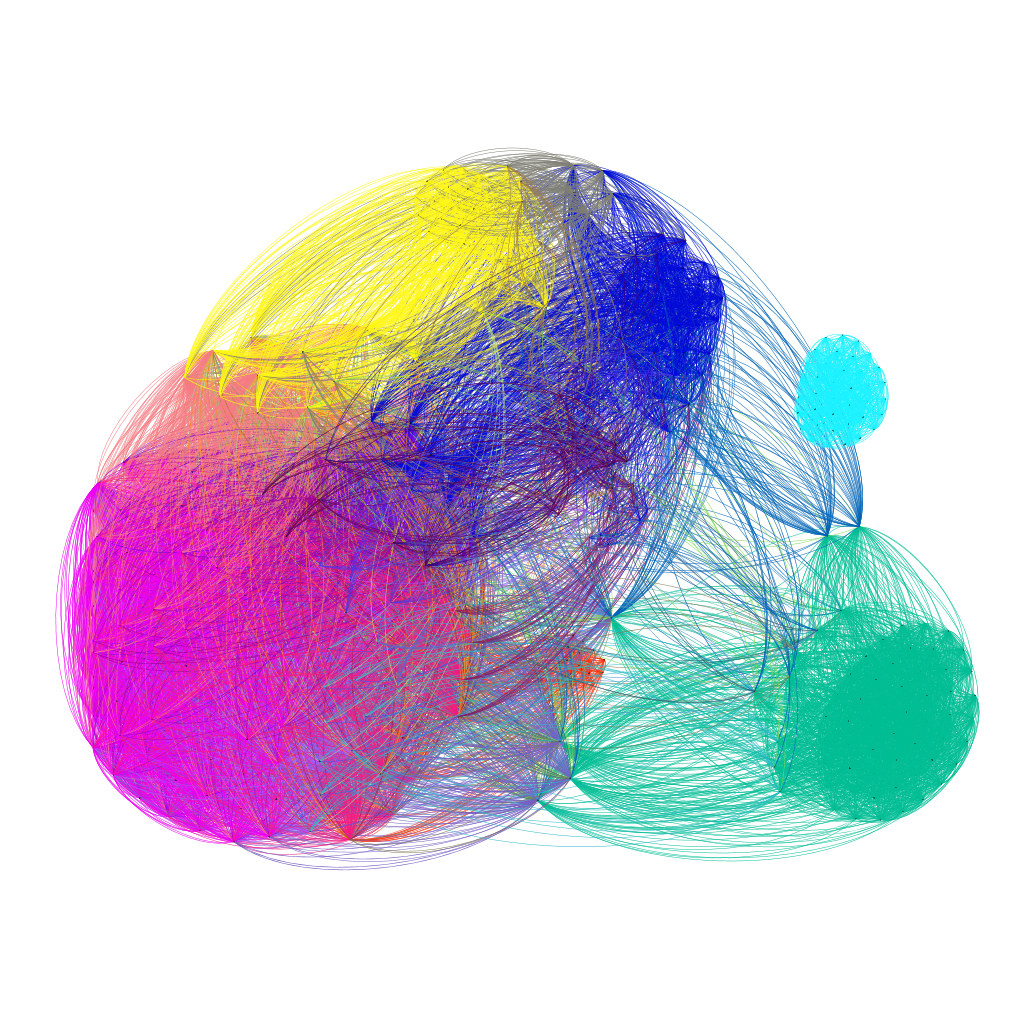
\includegraphics[width = 3.5in]{figures/Mexico_cluster1}}
%\caption{Mexico protests clustering results.}
%\label{Mexico-cluster}
%\end{figure}



%\begin{figure}[ht]
%\centerline
%{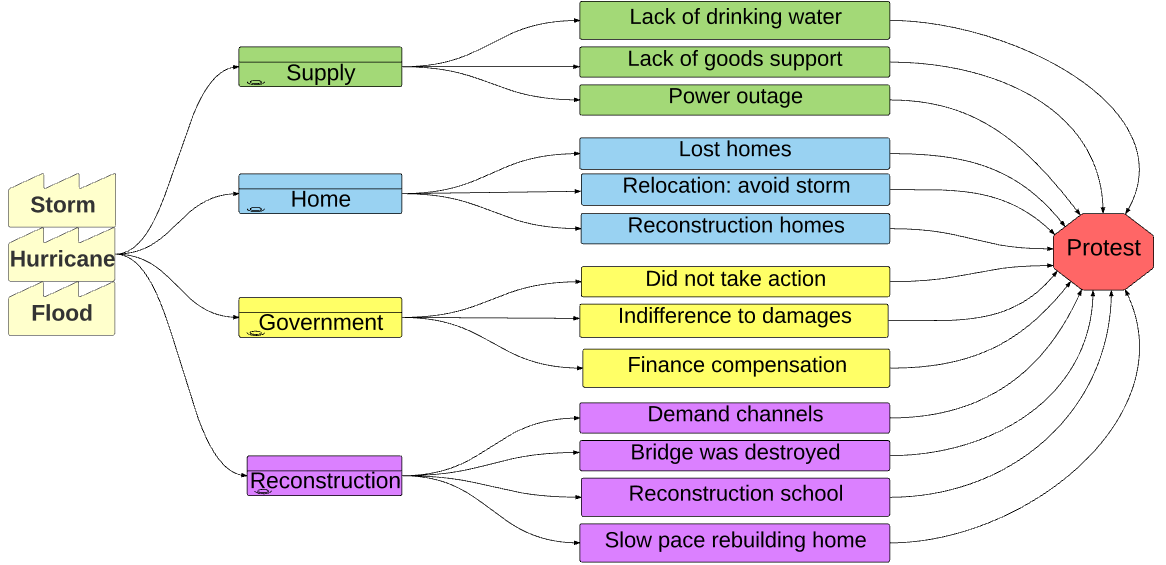
\includegraphics[height=1.4in]{figures/Mexico-diagram2}}
%\caption{Mexico climate protest causality diagram.}
%\label{Mexico-causality}
%\end{figure}
%
%
%\begin{figure}[ht]
%\centerline
%{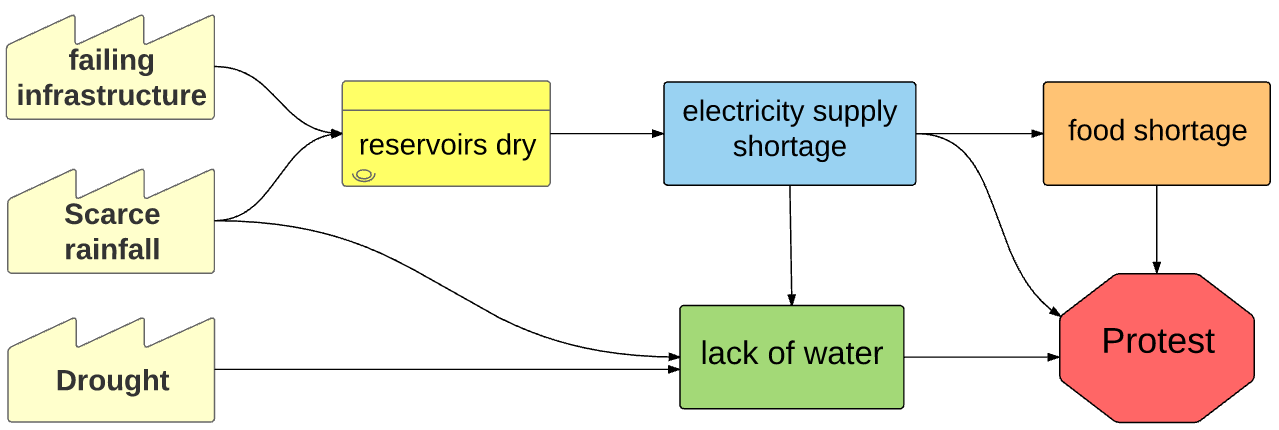
\includegraphics[height=1in, width=2.7in]{figures/Venezuela-diagram2}}
%\caption{Venezuela climate protest causality diagram.}
%\label{Venezuela-causality}
%\end{figure}
%
%\begin{figure}[ht]
%\centerline
%{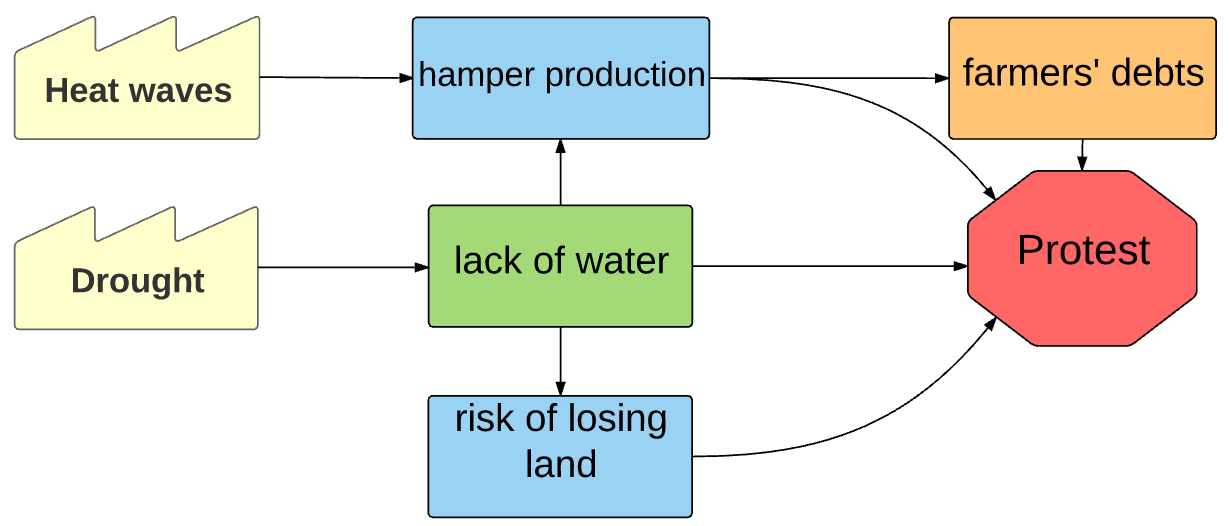
\includegraphics[height=1in, width=2.7in]{figures/Brazil-diagram}}
%\caption{Brazil climate protest causality diagram.}
%\label{Brazil-causality}
%\end{figure}


%\begin{figure}[ht]
%\centerline
%{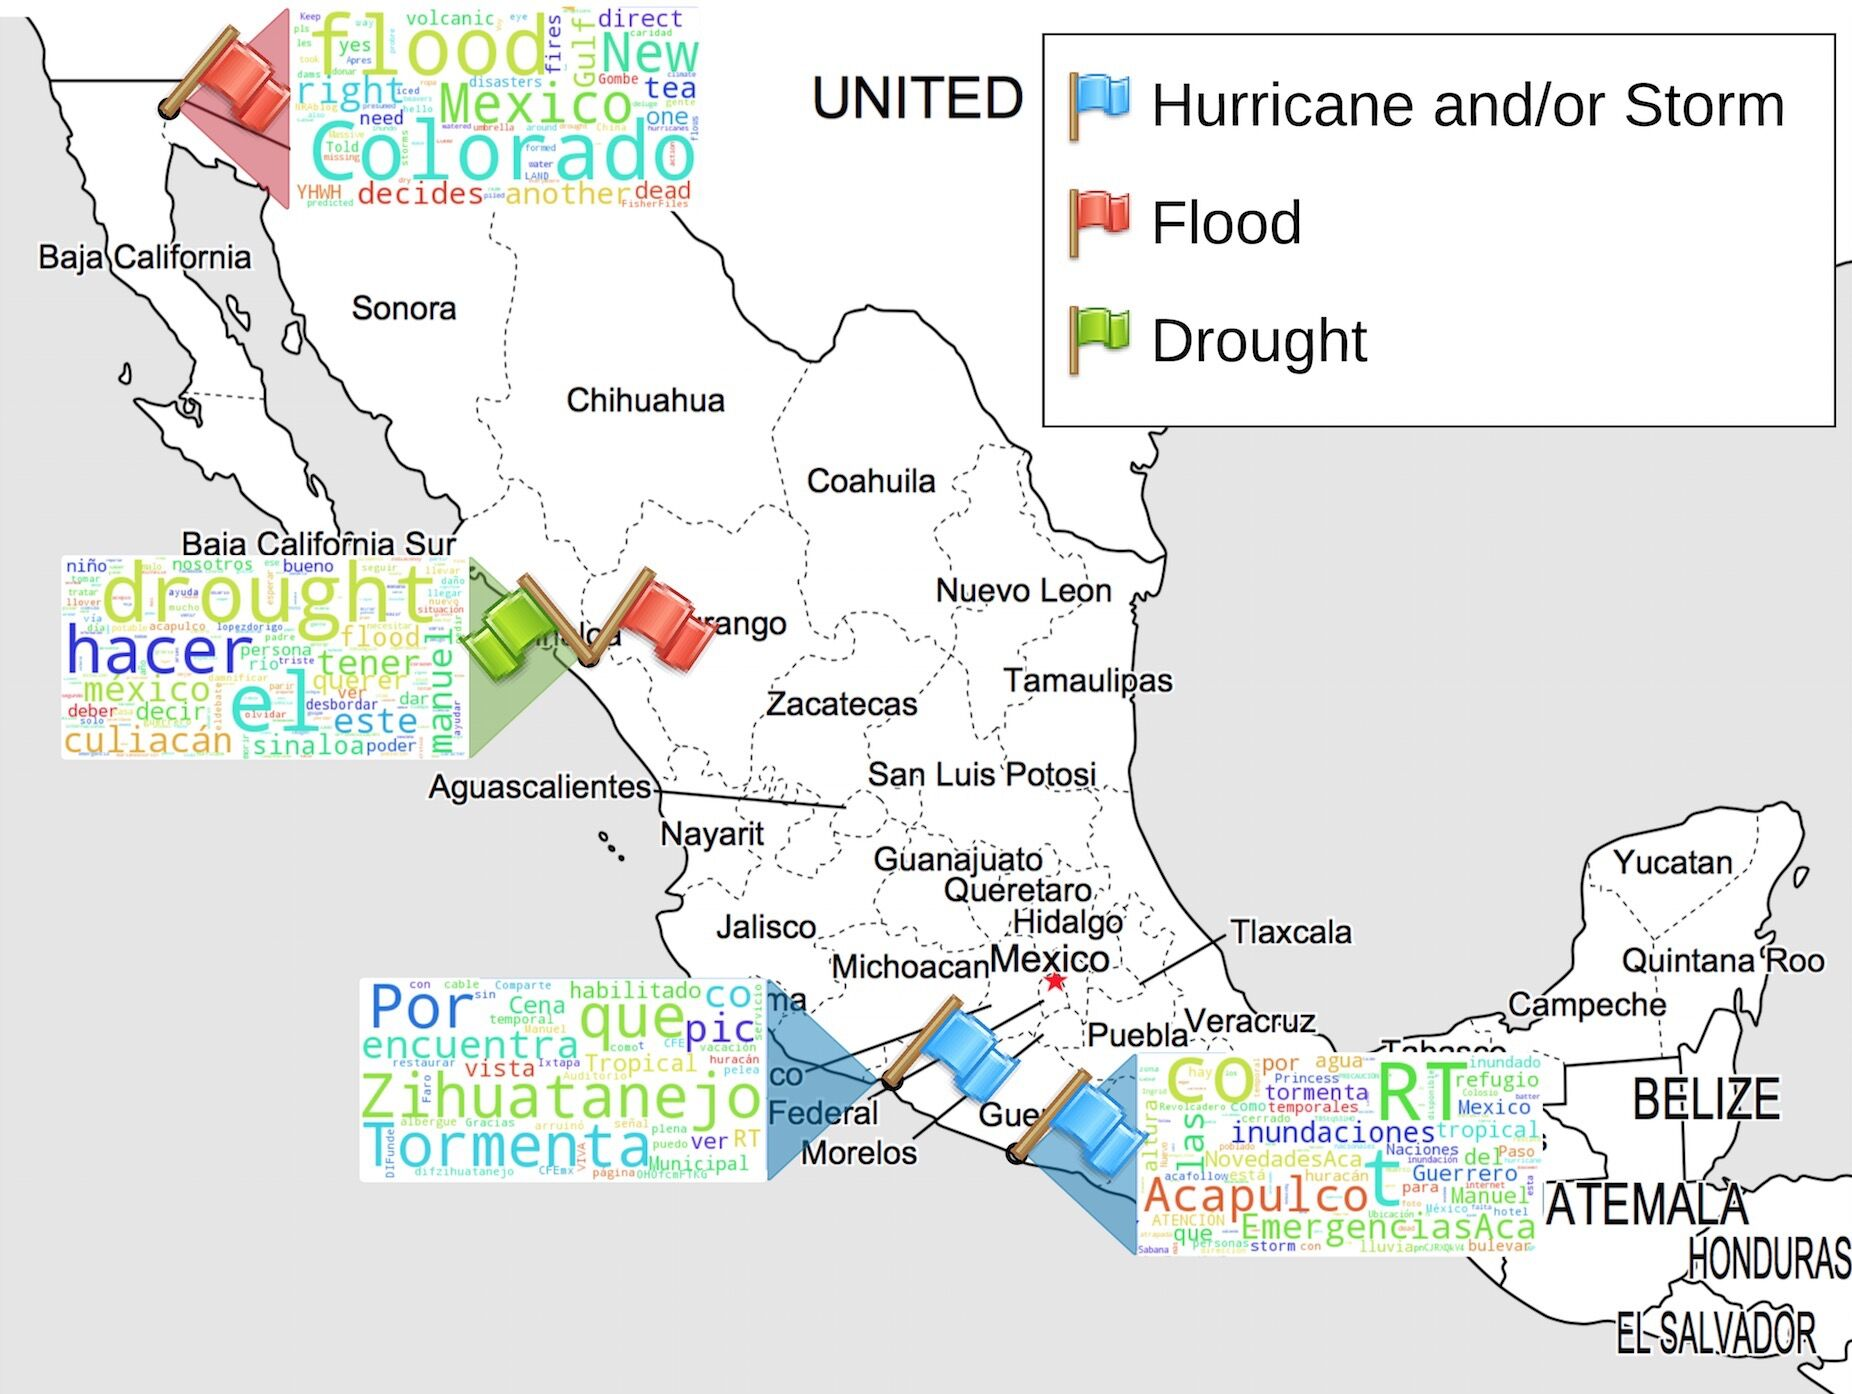
\includegraphics[width=.3\textwidth]{figures/Mexico-events}}
%\caption{Climate protest events in Mexico, Sept 2013. Different flag represents different climate disasters. The adjacent world cloud shows Twitter nnn as per that event.}
%\label{Mexico-events}
%\end{figure}
%
%
%\begin{figure}[ht]
%\centerline
%{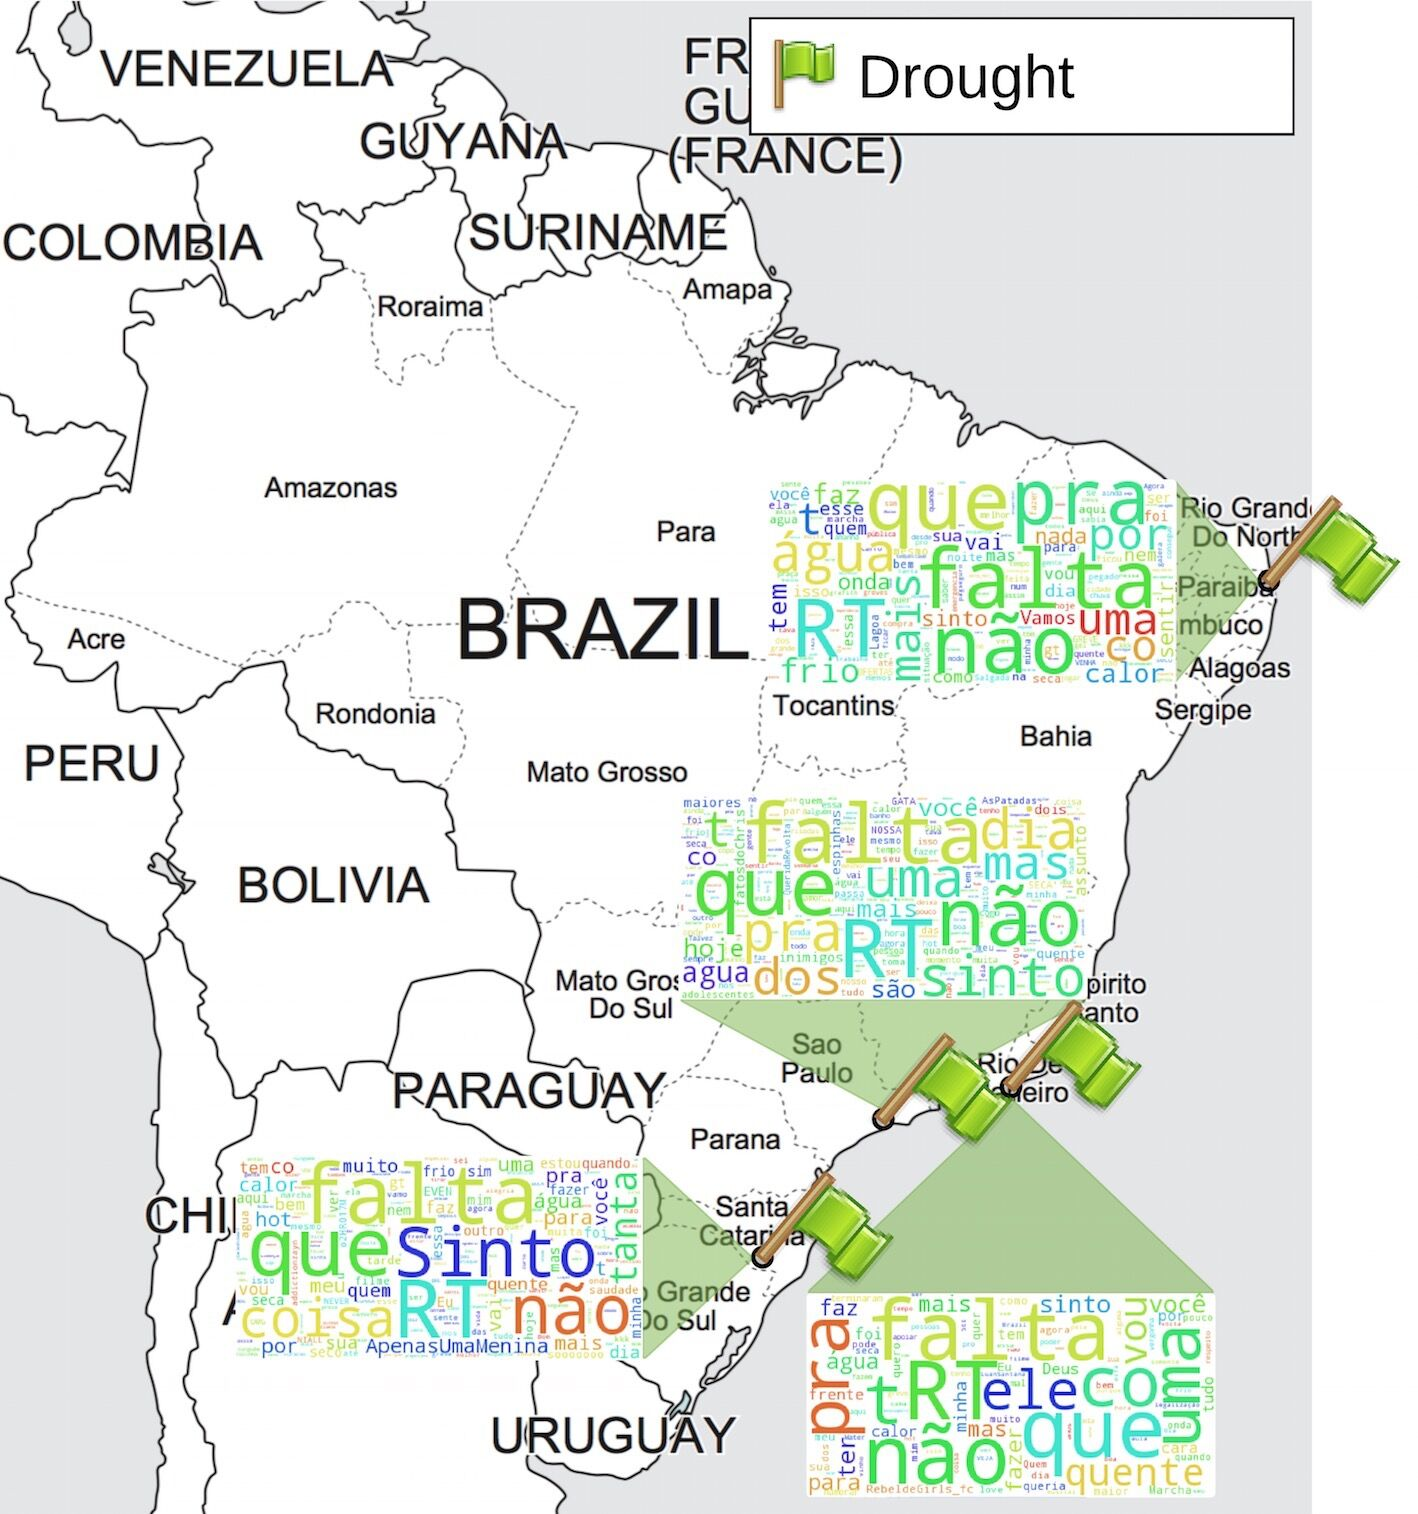
\includegraphics[width=.25\textwidth]{figures/Brazil-events}}
%\caption{Climate protest events in Brazil, May 2012. The adjacent world cloud shows Twitter discussion as per that event.}
%\label{Brazil-events}
%\end{figure}
%

%\begin{figure}[ht]
%\centerline
%{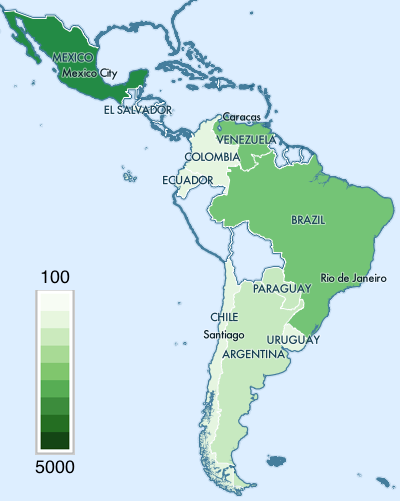
\includegraphics[width=.2\textwidth]{figures/GSR}}
%\caption{GSR protest events in Latin American countries, from November 2012 to August 2014.}
%\label{GSR}
%\end{figure}




%\begin{figure}[ht]
%\centerline
%{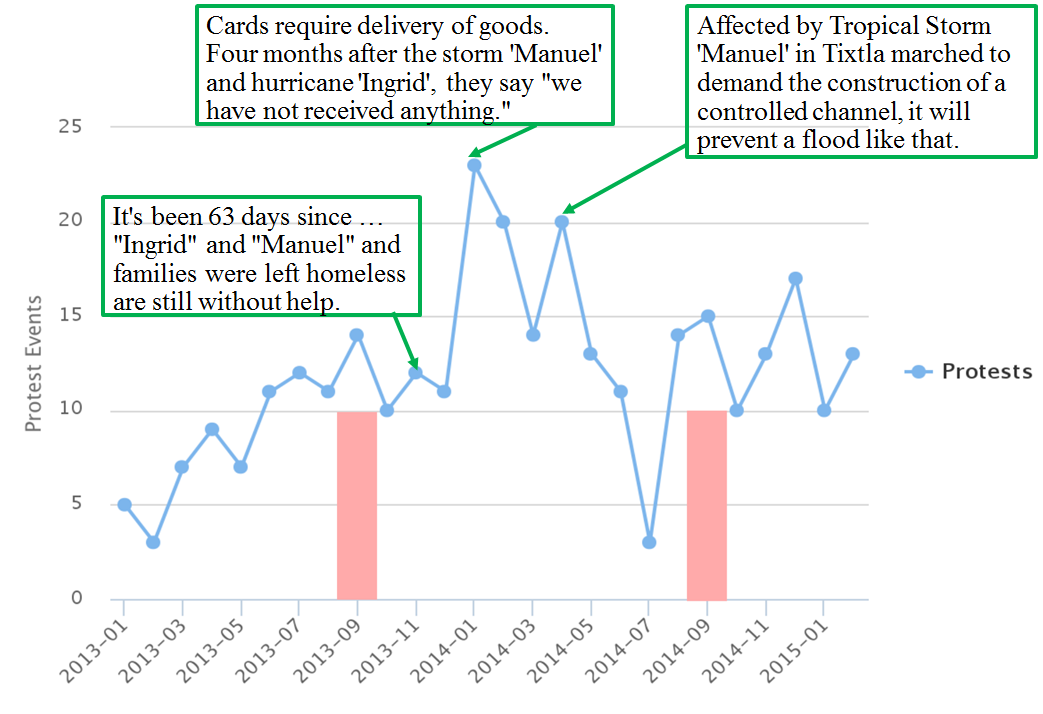
\includegraphics[width=.35\textwidth]{figures/Mexico_disaster2}}
%\caption{Mexico climate disasters and climate protests. The blue time series shows the climate related protest events, and light red vertical lines show two climate diasters in Mexico, storm Manuel in September 17, 2013 and hurricane Odile in September 15, 2014 respectively.}
%\label{Mexico_disaster_timeseries}
%\end{figure}
%
%
%\begin{figure}[ht]
%\centerline
%{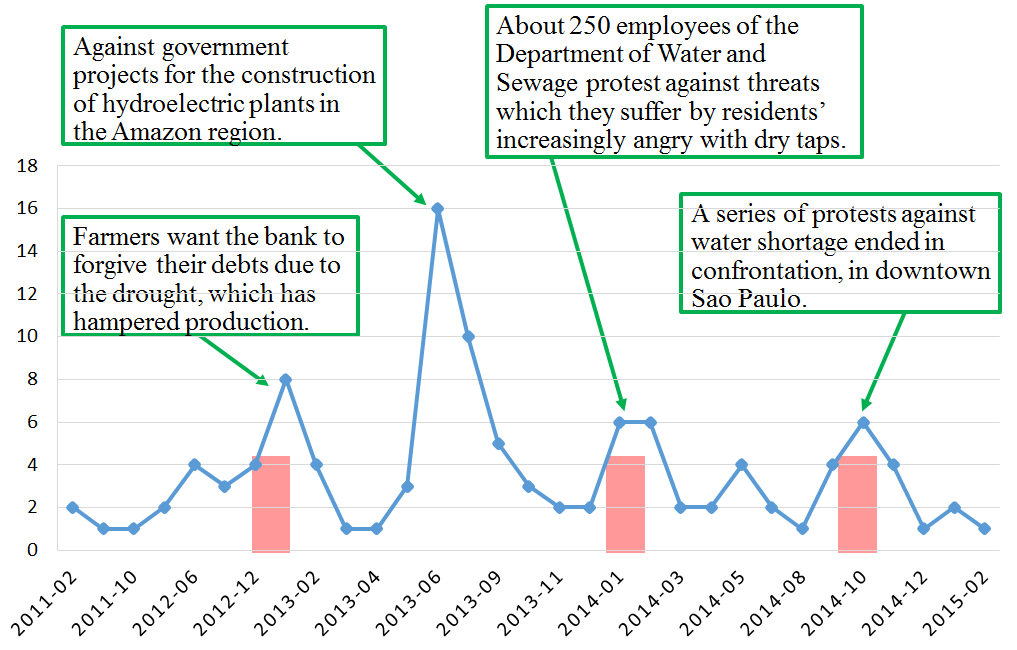
\includegraphics[width=.35\textwidth]{figures/Brazil_disaster1}}
%\caption{Brazil climate disasters and climate protests. The blue time series shows the climate related protest events, and light red vertical lines show three climate diasters in Brazil, drought in Feb 2012, Heat wave in Feb 2014, and drought in Oct 2014, respectively.}
%\label{Brazil_disaster_timeseries}
%\end{figure}
%
%
%
%\begin{figure}[ht]
%\centerline
%{\includegraphics[width=.4\textwidth]{figures/Venezuela_disaster}}
%\caption{Venezuela climate disasters and climate protests. The blue time series shows the climate related protest events, and light red vertical lines show flood diasters, and yellow vertical lines drought disasters.}
%\label{Venezuela_disaster_timeseries}
%\end{figure}

